%\documentclass[preprint]{aastex} 
\documentclass[iop,floatfix,numberedappendix,twocolappendix]{emulateapj} 

\usepackage[backref,breaklinks,colorlinks,urlcolor=blue,citecolor=blue,linkcolor=blue]{hyperref}
\usepackage[all]{hypcap}
\renewcommand*{\backref}[1]{[#1]}
\usepackage{graphicx}
%\usepackage{apjfonts}
\usepackage{enumerate}
\usepackage{amsmath,amssymb}
\usepackage{bm}
\usepackage{color}
\usepackage[utf8]{inputenc}

%version-control tagging based off of github.com/bd-j/speccal
%%% This file is generated by Makefile.
\newcommand{\githash}{b3f5d1c}\newcommand{\gitdate}{2014-08-19}\newcommand{\gitauthor}{Ian Czekala}

\newcommand{\prob}{{\rm prob}}
\newcommand{\qN}{\{q_i\}_{i=1}^N}
\newcommand{\qM}{\{q_{im}\}_{i=1,m=0}^{N,M}}
\newcommand{\yN}{\{y_i\}_{i=1}^N}

\newcommand{\kms}{ \textrm{km s}^{-1} }

\newcommand{\vM}{\mathsf{M}}
\newcommand{\vD}{\mathsf{D}}
\newcommand{\vR}{\mathsf{R}}
\newcommand{\vC}{\mathsf{C}}
\newcommand{\fM}{ \vec{{\bm M}}}
\newcommand{\fMi}{M_i}
\newcommand{\fD}{ \vec{{\bm D}}}
\newcommand{\fDi}{D_i}
\newcommand{\fR}{ {\bm R}}
\newcommand{\dd}{\,{\rm d}}
\newcommand{\trans}{\mathsf{T}}
\newcommand{\Z}{[{\rm Fe}/{\rm H}]}
\newcommand{\A}{[\alpha/{\rm Fe}]}
\newcommand{\matern}{Mat\'{e}rn}
\newcommand{\HK}{$\textrm{H}_2$O-K2}
\newcommand{\cc}[2]{c_{#2}^{(#1)}} 

\newcommand{\flam}{f_\lambda}
\newcommand{\vt}{ {\bm \theta}}
\newcommand{\vT}{ {\bm \Theta}}
\newcommand{\vp}{ {\bm \phi}}
\newcommand{\vP}{ {\bm \Phi}}
\newcommand{\cheb}{ \vp_{\mathsf{P}}}
\newcommand{\chebi}[1]{ \vp_{\textrm{Cheb}_{#1}}}
\newcommand{\Cheb}{ \vP_{\textrm{Cheb}}}
\newcommand{\Chebi}[1]{ \vP_{\textrm{Cheb}_{\ne #1}}} 
\newcommand{\cov}{ \vp_{\mathsf{C}}}
\newcommand{\covi}[1]{ \vp_{\textrm{cov}_{#1}}} 
\newcommand{\Cov}{ \vP_{\textrm{cov}}}
\newcommand{\Covi}[1]{ \vP_{\textrm{cov}_{\ne #1}}} 

\newcommand{\allParameters}{\vT} 
\newcommand{\nuisanceParameters}{\vP} 

\newcommand{\KK}{\mathcal{K}}
\newcommand{\Kglobal}{\KK^{\textrm{g}}}
\newcommand{\Klocal}{\KK^l}


\newcommand{\todo}[1]{ \textcolor{blue}{\\TODO: #1}}
\newcommand{\comm}[1]{ \textcolor{red}{SA: #1}}
\newcommand{\hili}[1]{ \textcolor{green}{#1}}
\newcommand{\ctext}[1]{ \textcolor{blue}{\% #1}}

\shorttitle{Robust Spectroscopic Inference with Imperfect Models}
\shortauthors{Czekala et al.}

\begin{document}

\graphicspath{{figs/}}

\slugcomment{draft: \today{}}


\title{Robust Spectroscopic Inference with Imperfect Models}

\author{Ian Czekala, Sean M.~Andrews, et al.}
\affil{Harvard-Smithsonian Center for Astrophysics, 60 Garden Street, Cambridge, MA 02138}
\email{iczekala@cfa.harvard.edu}

\begin{abstract}
We present a modular, extensible framework for the spectroscopic inference of 
physical parameters based on synthetic model spectra.  The subtraction of an 
imperfect model from a continuously sampled spectrum introduces covariance 
between adjacent datapoints (pixels) into the residual spectrum.  In the limit 
of high signal-to noise data with large spectral range that is common for 
stellar parameter estimation, that covariant structure can bias the parameter 
determinations.  We have designed a likelihood function formalism to account 
for the structure of the covariance matrix, utilizing the machinery of Gaussian 
process kernels.  We specifically address the common problem of mismatches in 
model spectral line strengths (with respect to data) due to intrinsic model 
imperfections (e.g., in the atomic or molecular data, or radiative transfer 
treatment) by developing a novel local covariance kernel framework that 
identifies and self-consistently downweights pathological spectral line 
``outliers."  By fitting multiple spectra in a hierarchical manner, these local 
kernels provide a mechanism to learn about and build data-driven corrections to 
synthetic model spectral libraries.  The application of this method, 
implemented as a freely available open source code, is demonstrated by fitting 
the high resolution optical ($V$-band) spectrum of WASP-14, an F5 dwarf with a 
transiting exoplanet, and the moderate resolution near-infrared ($K$-band) 
spectrum of Gliese~51, an M5 dwarf. 
\end{abstract}
\keywords{stars: fundamental parameters --- methods: data analysis --- methods: statistical}




\section{Introduction} \label{sec:intro}

All astronomers recognize that spectroscopy offers a wealth of information that 
can help characterize the properties of the observing target.  In the context 
of stellar astrophysics, spectroscopy plays many fundamental roles.  The 
relative strengths and widths of stellar absorption lines provide access to key 
parameters like effective temperature ($T_{\rm eff}$) and surface gravity 
($\log g$), enabling model comparisons in the Hertzsprung-Russell diagram to 
estimate the masses and ages so crucial to understanding stellar evolution, as 
well as individual elemental (and molecular) abundances or the collective 
``metallicity" (typically parameterized as [Fe/H]), facilitating study of the 
chemical hallmarks of different stellar populations.  With sufficient spectral 
resolution, the velocity content of a spectrum can convey crucial information 
about stellar rotation ($v \sin i$) and kinematics (e.g., association with a 
cluster or companion through the radial velocity, $v_z$).  While many fields 
benefit from the spectroscopic measurements of these stellar properties, there 
is acute interest in the exoplanet community.  There, all estimates of the 
planet properties are made {\it relative} to the host properties (e.g., the 
planet-to-host mass or radius {\it ratio} is constrained with the radial 
velocity or transit techniques, respectively).  Moreover, essential clues to 
the planet formation process are encapsulated in the dependences of planet 
frequency on host mass \citep[e.g.,][]{johnson07,howard10} and metallicity 
\citep[e.g.,][]{fischer05,buchhave14}.   

That said, the robust and quantitative extraction of physical (or empirical) parameters from an 
observed spectrum can be an extraordinary challenge.  Stellar models are ultimately required as a 
comparative benchmark to associate observed spectral features with the parameters of interest.  
Generating a synthetic model spectrum requires a complex numerical treatment of the stellar 
structure and radiative transfer through the atmosphere \citep[e.g.,][]{kurucz93,castelli04,
hauschildt99,husser13,paxton11}.  Detailed models calibrated to individual stars are important, but 
rare (e.g., the Sun, Vega); as such, these stellar models are relatively untested in large swaths 
of parameter-space.  Moreover, they necessarily include simplifications to treat complicated 
physical processes (e.g., convection) or computational limitations (e.g., geometry, boundary 
conditions), and often must rely on incomplete or inaccurate atomic and molecular information 
(e.g., oscillator strengths, opacities).  In principle, the models could be further improved with 
appropriate reference to spectroscopic datasets.  Nevertheless, they achieve a remarkable level of 
success in reproducing many key diagnostic features in stellar spectra.  

There are various well-tested techniques being used to compare these models with observed spectra 
and thereby infer basic stellar parameters; here we highlight three examples to illustrate some key 
ideas.  First is a straightforward empirical approach that relies on distilling an information-rich 
subset of the data, usually in the form of spectral line equivalent widths and/or local continuum 
shapes.  A combined sequence of the ratios of these quantities are found to be especially sensitive 
to one key parameter in the models, and therefore can be used to quantify it \citep[e.g., {\tt 
MOOG};][]{sneden73,gray94,reid95,rojas-ayala10,rojas-ayala12}.  This ``indexing" approach has the 
advantage of being trivially fast, but each condensed relationship is only informative over a 
limited swath of parameter-space.  A second technique exploits the cross-correlation of a spectrum 
with a suite of model templates to optimize a set of parameters, usually with some weighting 
applied to specific spectral regions \citep[e.g., {\tt SPC};][]{buchhave12}.  In this case, the 
speed advantage is maintained (perhaps enhanced) and more data content is used (particularly in the 
spectral dimension), thereby achieving higher precision even for data with comparatively low 
sensitivity; the disadvantage is that the model quality and parameter inferences are assessed in an 
empirical, rather than probabilistic, framework.  A third approach employs a direct, pixel-by-pixel 
comparison between model and data, and is usually associated with a spectral synthesis back-end 
(e.g., {\tt SME}; \citealt{valenti96}).  This technique has the benefits of parametric flexibility 
(e.g., one can fit for arbitrary abundances or structures) and a proper inference framework 
\citep[usually a least-squares approach, although increasingly in a Bayesian format;][]{shkedy07,
schoenrich13}, but it is computationally expensive and can be biased by systematics 
\citep[e.g.,][]{mann13}; in practice, this often requires an effort focused on a pre-selected 
subsample of the data. 

In this article, we design a flexible forward-modeling approach to the general spectroscopic 
inference problem in a Bayesian framework, building on the best aspects of the latter two methods 
highlighted above.  Employing a non-trivial covariance matrix parameterized by both global 
(stationary) and local (non-stationary) Gaussian process kernels, we are able to account for 
residual pixel-to-pixel correlations that arise when comparing observed spectra to intrinsically 
imperfect models.  This approach minimizes the potential for bias, efficiently propagates 
systematic uncertainties into the parameter inferences, and ultimately can serve as a tool for 
using observations to guide substantial improvements in the models themselves.  An overview of the 
methodology of this approach is provided in Section \ref{sec:method}, including the covariance 
matrix formalism.  Some tests and example applications (for a high resolution optical spectrum of 
an F star, and a medium-resolution near-infrared spectrum of a mid-M star) of the method are 
described in Section \ref{sec:examples}.  Finally, a discussion of the potential utility of the 
technique, and the possibility of extending it to develop data-driven spectral models, is provided 
in Section \ref{sec:discussion}.  \\



\section{Methodology} \label{sec:method}

In this Section, we describe a generative Bayesian modeling framework that confronts some of the 
key obstacles in the spectroscopic inference problem.  The goal of this approach is to 
conservatively extract the maximal amount of information about a prescribed (and usually 
degenerate) parameter set by forward-modeling an observed spectrum, while also recognizing and 
explicitly accounting for the covariances and biases introduced by pathologically imperfect 
models.  The method is modular, and therefore can easily incorporate additional physical or 
nuisance parameters as desired without sacrificing an accurate reflection of the limitations in the 
data.  Moreover, with a well-crafted observational sample, this data-driven approach should 
ultimately enable us to systematically learn how synthetic spectral models can be improved.  The 
specific applications discussed here are related to the spectra of individual stars, but the 
methodology is generic (and could be used for the composite spectra of unresolved stellar clusters, 
galaxies, etc.).  

The remainder of this Section describes the mechanics of this modeling framework.  First, a model 
spectrum is generated for a given set of physical parameters (Section \ref{subsec:synthetic}; 
Appendix~\ref{sec:Appendix}), and then post-processed to mimic reality using a set of observational 
and practical nuisance parameters (Section \ref{subsec:postprocess}).  Next, a direct, 
pixel-by-pixel comparison between the data and model spectra is made with a prescribed likelihood 
function and a parametric treatment of the covariances between pixel residuals (Section 
\ref{subsec:likelihood}).  That process is iterated under the guise of hierarchical Markov Chain 
Monte Carlo (MCMC) simulations to numerically explore the posterior probability density of the 
model conditioned on the data, and thereby to determine constraints on the parameters of interest 
(Section \ref{subsec:MCMC}).  Along the way, these procedures are illustrated with observations of 
the high resolution optical spectrum from a nearby F star.  That specific application, along with 
some alternative demonstrations of the method, are discussed in more detail in Section 
\ref{sec:examples}.


\subsection{Generating a Model Spectrum \label{subsec:synthetic}}

There are various approaches to synthesizing a spectrum, $f_{\lambda}$, for a specific set of model
parameters, $\vt_{\ast}$.  In an ideal case, a model stellar atmosphere is constructed and then 
subsequently processed through a radiative transfer code \citep[e.g.,][]{kurucz93,hauschildt99}.  
However, in general this approach is still computationally prohibitive for any iterative method of 
probabilistic inference.  One partial compromise is to interpolate over a library of atmosphere 
structures that were pre-computed for a discrete grid of parameter values, $\{\vt_{\ast}\}^{\rm 
grid}$, for some arbitrary $\vt_{\ast}$, and then perform a radiative transfer calculation with 
that interpolated atmosphere to synthesize $\flam$ \citep[e.g., as for {\tt SME};][]{valenti96}.  A 
more common variant is to instead rely on interpolation over a library of pre-synthesized model 
spectra, $\flam(\vt_{\ast})$ \citep[e.g.,][]{castelli04,allard12,husser13}.  While technically the 
former approach is most similar to the ideal case, the computational cost of repeated spectral 
synthesis is sufficiently high to make a detailed exploration of parameter space (particularly for 
data with a large spectral range) considerably less appealing.  An alternative approach eschews 
forward modeling entirely (and therefore repeated spectral syntheses and/or library 
interpolations), and instead evaluates the models only at the discrete grid points of the library.  
Then, these discretized samples of the posterior probability density can be interpolated to an 
arbitrary $\vt_{\ast}$ to construct appropriate confidence intervals \citep[similar to the method 
of {\tt SPC};][]{buchhave12}.  The difficulty with this latter approach is that the parameter 
uncertainties can be smaller than the grid spacing; in that case, there is valid concern that this 
interpolation might not accurately recover intrinsic parameter degeneracies.

We opt for the computationally expedient approach that employs a library of model spectra, 
$\flam(\{\vt_{\ast}\}^{\rm grid})$, where $\vt_{\ast} = [T_{\rm eff}, \,\, \log{g}, \,\, 
[{\rm Fe/H}]]$.  However, it is worth noting that the techniques developed here are applicable to 
{\it any} ``back-end" that generates a model spectrum.  In our adopted approach, the model spectrum 
for an arbitrary $\vt_{\ast}$ is interpolated from a spectral library,
\begin{equation} \label{eqn:interp} 
\flam(\{\vt_{\ast}\}^{\rm grid}) \leadsto \flam(\vt_{\ast}), 
\end{equation} 
where we assign the symbol $\leadsto$ as an interpolation operator.  The multi-dimensional 
interpolation in Eq.~\ref{eqn:interp} needs to be performed many times, so computational efficiency 
is critical.  In practice, a simple tri-linear interpolation is suitably fast, but introduces a 
non-negligible level of uncertainty.  These interpolation uncertainties can be empirically 
estimated by performing the operation in Eq.~\ref{eqn:interp} across a $\{\vt_{\ast}\}^{\rm grid}$ 
grid point, and then comparing the interpolated spectrum with the corresponding library spectrum 
\citep[see also][]{husser12}.  To suitably propagate the interpolation uncertainties into the 
likelihood calculations, we employ a Bayesian emulation technique that is described in detail in 
Appendix \ref{sec:Appendix}.


\subsection{Post-Processing} \label{subsec:postprocess}

Generally, the ``raw" model spectrum $\flam(\vt_{\ast})$ is highly over-sampled compared to the 
observed spectrum, and does not account for several additional observational and instrumental 
effects that become important in comparisons with real data.  Therefore, a certain amount of 
post-processing is required before assessing the model quality.  We treat that post-processing in 
two stages: the first deals with an additional set of ``observational" parameters, $\vt_{\rm obs}$, 
that incorporate dynamical effects, geometry, and the relative location of the target, while the 
second employs a suite of nuisance (hyper-)parameters ($\vp$) designed to mitigate an imperfect 
data calibration.

We can further divide $\vt_{\rm obs}$ into those parameters that impact the model primarily in the 
spectral or flux dimensions.  For the former, we consider three kernels that contribute to the 
line-of-sight velocity distribution function, $\varphi_v$.  The first, $\mathcal{F}_v^{\rm inst}$, 
treats the instrumental spectral broadening.\footnote{For computational efficiency, we first 
pre-convolve the entire raw spectral library with a slight under-prediction of $\mathcal{F}_v^{\rm 
inst}$ and resample the spectra to a lower resolution.  Because the instrumental point spread 
function acts as a low-pass filter, this procedure reduces the size of the library by a factor of 
10 or more while still preserving the final Fourier content of the spectra.  Then, when any given 
spectrum is post-processed, the actual $\mathcal{F}_v^{\rm inst}$ used is treated as a smaller 
``correction" to this pre-processing kernel.}  For illustrative purposes, we assume 
$\mathcal{F}_v^{\rm inst}$ is a Gaussian with mean $v = 0$ and constant width $\sigma_v$ at all 
$\lambda$, although more sophisticated forms could be adopted.  The second, $\mathcal{F}_v^{\rm 
rot}$, characterizes the broadening induced by (projected) stellar rotation, parameterized by 
$v\sin{i}$ as described by \citet[][his Eq.~18.14]{gray08}.  And the third, $\mathcal{F}_v^{\rm 
dop} = \delta(v-v_z)$, incorporates the radial velocity through a Doppler shift.  The model 
spectrum is modified by the parameters $[\sigma_v, \,\, v\sin{i}, \,\, v_z]$ through these kernels, 
using a convolution in velocity-space,\footnote{In practice, these convolutions are performed as 
multiplications in Fourier-space to better preserve spectral information \citep[cf.,][]{tonry79}; 
the mathematical formalism is presented for clarity.}
\begin{eqnarray} \label{eqn:broadening}
\flam(\vt_{\ast}, \sigma_v, v\sin{i}, v_z) &=& \flam(\vt_{\ast}) \ast \varphi_v \\
                                           &=& \flam(\vt_{\ast}) \ast \mathcal{F}_v^{\rm inst} \ast \mathcal{F}_v^{\rm rot} \ast \mathcal{F}_v^{\rm dop}, \nonumber
\end{eqnarray} 
and then re-sampled onto the discrete wavelengths corresponding to each data pixel, 
\begin{equation} \label{eqn:resampling}
\flam(\vt_{\ast},  \sigma_v, v\sin{i}, v_z) \mapsto \vM(\vt_{\ast},  \sigma_v, v\sin{i}, v_z),
\end{equation}
where the $\mapsto$ symbol denotes a re-sampling operator that maps the model spectrum onto the 
$N_{\rm pix}$-element model vector $\vM$ ($N_{\rm pix}$ is the number of pixels in the spectrum).  
Figure \ref{fig:broadening} shows a (condensed) graphical representation of these post-processing 
steps.

\begin{figure}[!t]
\begin{center}
  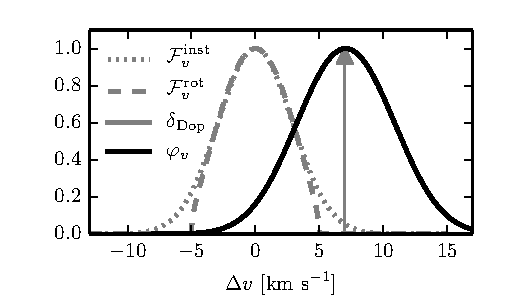
\includegraphics{figs/kernels.pdf}
  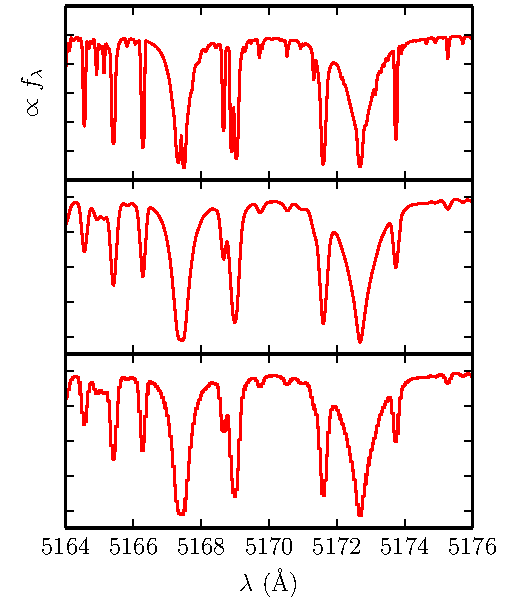
\includegraphics{figs/high2low.pdf}
  \figcaption{({\it top}) The line-of-sight velocity distribution function, $\varphi_v$, and its 
decomposition into broadening kernels.  The instrumental kernel ({\it dotted}) is treated as 
a Gaussian, the rotation kernel ({\it dashed}) is a Gaussian-like function of the projected 
rotational velocity, and the Doppler kernel ({\it solid}) is a $\delta$-function that introduces 
the radial velocity.  In this specific case, $\sigma_v = 2.9$\,km s$^{-1}$, $v\sin{i} = 5$\,km 
s$^{-1}$, and $v_z = 7$\,km s$^{-1}$, appropriate for the example in Section \ref{subsec:wasp}.
({\it bottom}) A segment of a raw, full-resolution model spectrum and its post-processed equivalent 
after convolution by $\varphi_v$ and re-sampling at the coarser resolution of the detector pixels. 
\label{fig:broadening}}
\end{center}
\end{figure}

At this stage, the model is further modified in the flux dimension.  A typical synthetic spectrum 
is computed as the flux that would be measured {\it at the stellar surface}, and so needs to be 
diluted by the subtended solid angle, $\Omega = (R_{\ast}/d)^2$, where $R_{\ast}$ is the stellar 
radius and $d$ is the distance.  An additional wavelength-dependent scaling factor is applied to 
account for interstellar extinction, assuming some previously-derived extinction law $A_{\lambda}$ 
\citep[e.g.,][]{cardelli89} that is parameterized by $A_V$.  The parameters $[\Omega, \,\, A_V]$ 
are then applied as
\begin{eqnarray} \label{eqn:scaling}
\vM(\vT) &=& \vM(\vt_{\ast}, \vt_{\rm obs}) \\
         &=& \vM(\vt_{\ast}, \sigma_v, v\sin{i}, v_z) \times \Omega \times 10^{-0.4\,A_{\lambda}}, \nonumber
\end{eqnarray}
with simplified notation such that $\vT \equiv [\vt_{\ast}, \,\, \vt_{\rm obs}]$, 
where $\vt_{\rm obs} = [\sigma_v, v\sin{i}, v_z, \Omega, A_V]$.

% NEEDS UPDATED FIGURE
\begin{figure}[b!]
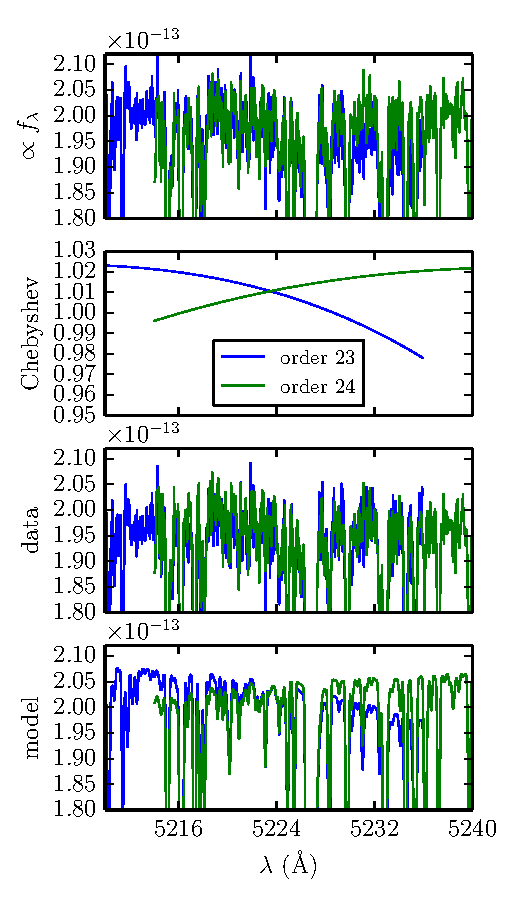
\includegraphics{figs/chebyshev.pdf}
\vspace{-0.75cm}
\figcaption{A demonstration of our treatment for residual calibration mismatches.  The observed 
spectra at the overlap of two echelle orders ({\it top}) have slightly ($\sim$1--3\%) discrepant 
shapes.  Chebyshev polynomials ({\it middle, top}) are designed to account for that mismatch ({\it 
middle, bottom}); rather, in practice, the model is scaled (multiplied) by those polynomials ({\it 
bottom}).  \label{fig:chebyshev}}
\end{figure}

The procedure so far, summarized in Eq.~\ref{eqn:interp}--\ref{eqn:scaling}, is composed of 
straightforward operations demanded by practical astronomical and computing issues.  If the data 
were {\it perfectly} calibrated, we could proceed to a likelihood calculation that makes a direct 
comparison with $\vM(\vT)$.  However, that is unlikely to be the case.  The key concern is that an 
imperfect calibration might produce mismatches in the underlying shapes of the data and model.  
Although such mismatches presumably occur at a low-level over relatively broad wavelength scales, 
they still might represent a non-trivial likelihood contribution, and thereby bias our estimates of 
the physical parameters.  This issue is usually treated externally to any modeling procedure, most 
often by dividing the observed spectrum (and model spectrum) by a polynomial in $\lambda$.  But 
that ``normalization" implicitly assumes that there is no relevant information content in the 
spectral shape; if $\vT$ also contributes on the mismatched scales, then adopting this approach 
will corrupt the inferences of these parameters.  Moreover, in practice this approach is limited, 
since defining an appropriate polynomial becomes difficult in cases where the spectral line density 
is high (e.g., molecular bands for cool stars).  

We employ an analogous, but more rigorous, approach to deal with this issue, cast {\it internal} to 
the modeling framework to propagate the uncertainties introduced by additional degrees of freedom 
in the model.  Deviations in the spectral shape introduced by calibration residuals are treated as 
explicit contributions to the model spectrum, enabling an exploration of the distribution of 
possible ``tweaks" to the calibration that can be compartmentalized into a set of nuisance 
parameters and then marginalized.  This way, the inferences for the stellar parameters will 
properly account for the underlying uncertainty in the calibration of the spectral shape.  In 
practice, this is achieved by distorting segments of the model spectrum with polynomials, 
$\mathsf{P}$ \citep[e.g.,][]{eisenstein06,koleva09}.  For data that has $N_{\rm ord}$ spectral 
orders, each denoted with index $o$, the model spectrum can be decomposed into the set of orders
\begin{eqnarray} \label{eqn:chebyshev}
\vM(\vT, \cheb) &=& \{ \vM_o(\vT) \times \mathsf{P}_o \} \\
                &=& \{ \vM_o(\vT) \times \sum_n c_o^{(n)} \, T_o^{(n)} \}, \nonumber
\end{eqnarray}
where $T^{(n)}$ is an $n^{\rm th}$ degree Chebyshev function.  The $n \times N_{\rm ord}$ 
coefficients are considered a set of nuisance (hyper-)parameters, $\cheb = [\{c_o^{(0)}, c_o^{(1)}, 
\ldots, c_o^{(n-1)} \}]$.  With judicious priors, we can ensure that the unintended treatment of 
real spectral features (e.g., molecular bands) as residual calibration artifacts is negligible.  
The lowest-degree (scaling) coefficient, $c^{(0)}$, is naturally degenerate with the solid angle, 
$\Omega$.  Therefore, we enforce an additional constraint that the mean of the polynomial is 
unity.  For data with a single spectral order, this means simply setting $c^{(0)} = 1$.  In the 
multiple order case, we assign $c^{(0)} = 1$ in an arbitrary order as an anchor, but permit the 
$c^{(0)}$ in other orders to be different.  Figure \ref{fig:chebyshev} offers a practical 
demonstration of how these nuisance parameters are applied to the model. 


\subsection{Model Evaluation} \label{subsec:likelihood}

The quality of the model spectrum is assessed by comparing to the data with a pixel-by-pixel 
likelihood calculation.  If we denote the data spectrum as $\vD$, then a corresponding residual 
spectrum (an $N_{\rm pix}$-element vector) can be defined for any input parameter set,
\begin{equation}
\vR \equiv \vR(\vT, \cheb) \equiv \vD-\vM(\vT, \cheb).
\end{equation}
To quantify the probability of the data conditioned on the model, we adopt a standard 
multi-dimensional Gaussian likelihood function
\begin{equation}
p(\vD|\vM) =  \frac{1}{[(2 \pi)^{N_{\rm pix}} \det(\vC)]^{1/2}} \exp\left ( -\frac{1}{2} \,
   \vR^\trans \vC^{-1} \vR \right )
   \label{eqn:likelihood}
\end{equation}
that penalizes models which yield larger residuals and explicitly allows for covariances in the 
residual spectrum through the $N_{\rm pix} \times N_{\rm pix}$ matrix $\vC$.  For practical 
reasons, the log-likelihood is used as the quality metric, where
\begin{equation}
  \ln{p(\vD | \vM)} = -\frac{1}{2} \left( \vR^\trans \vC^{-1} \vR + \ln{\det{\vC}} + N_{\rm pix} \ln{2\pi} \right).
  \label{eqn:lnlikelihood}
\end{equation}

The covariance matrix $\vC$ characterizes both the measurement uncertainty ($\sigma$; ``noise") in 
each pixel and the intrinsic covariance between pixels.  The special case where each pixel 
represents an independent measurement results in a diagonal covariance matrix, $\vC_{ij} = 
\delta_{ij} \,\, \sigma_i$ where $\sigma_i$ is the uncertainty in pixel $i$ and $\delta_{ij}$ is 
the Kronecker delta function, and Eq.~\ref{eqn:lnlikelihood} reduces to the familiar
\begin{equation}
\ln{p(\vD | \vM)} = -\frac{1}{2} \sum_i^{N_{\rm pix}} \frac{\vR_i^2}{\sigma_i^2} \equiv -\frac{\chi^2}{2},
\label{eqn:chisq}
\end{equation}
the sum of the square of the residuals weighted by their inverse variances.  However, the problem 
being addressed here necessitates the use of a more complex covariance matrix; additional 
off-diagonal terms that can explicitly characterize (1) pixel-to-pixel covariances imposed by the 
discrete over-sampling of the line-spread function, and (2) highly correlated residuals as 
manifestations of the still-imperfect model library are required to avoid biasing our inferences of 
the physically interesting parameters ($\vT$).  The following subsections describe how these issues 
are addressed in the practical implementation of $\vC$.  


\subsubsection{Global Covariance Structure} \label{subsec:global_covariance}

Astronomical spectrographs are designed such that the detector over-samples the instrumental 
line-spread function with at least a few pixels.  Therefore, adjacent pixels never record 
independent samples of the true spectrum.  In that case, a difference between an observed and 
modeled spectral feature will create a correlated residual that spans multiple pixels.  This can be 
demonstrated practically through the autocorrelation of $\vR$: a slight model mismatch will produce 
correlated residuals over a characteristic scale similar to the instrumental broadening kernel 
width ($\sigma_v$).  Figure \ref{fig:class0} highlights a specific example of these correlated 
residuals in real data; a significant autocorrelation signal is found on a $\sim$5 pixel scale, 
corresponding to the 6.8\,km s$^{-1}$ FWHM of $\mathcal{F}_v^{\rm inst}$.  

\begin{figure}[!htb]
\begin{center}
  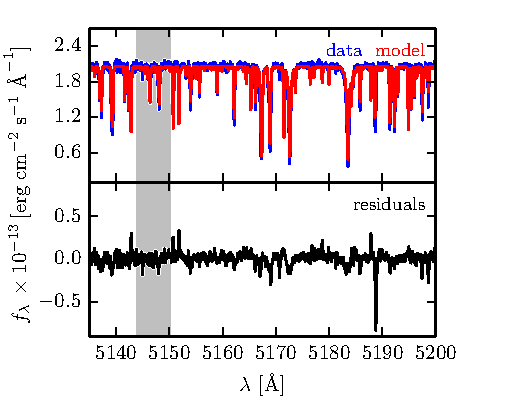
\includegraphics{residuals_23.pdf}
  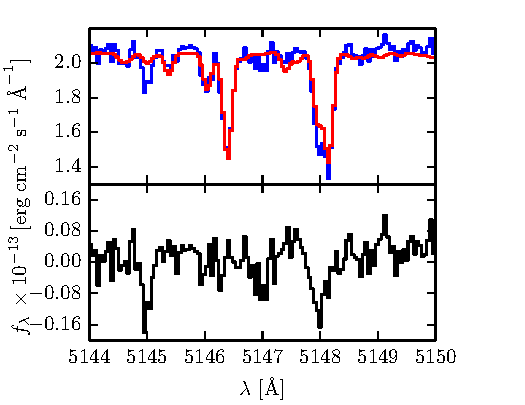
\includegraphics{class0_residuals.pdf}
  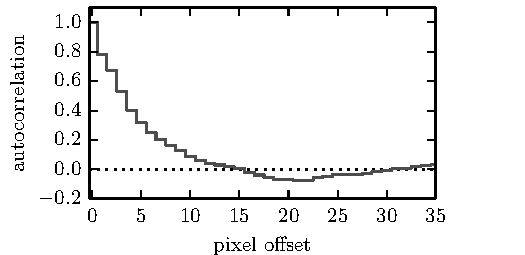
\includegraphics{class0_autocorrelation.pdf}
  \figcaption{({\it top}) A comparison of the data and a typical model with parameters drawn from 
the posterior distribution, along with the corresponding residual spectrum.  ({\it middle}) A 
zoomed view of the gray band in the top panels, highlighting the mildly covariant residual 
structure that is produced by slight mismatches between the data and model spectra.  ({\it bottom}) 
The autocorrelation of the residual spectrum.  Notice the substantial autocorrelation signal for 
offsets of $\lesssim 8$ pixels, demonstrating clearly that the residuals are not described well by 
white (Poisson) noise alone. \label{fig:class0}}
\end{center}
\end{figure}

It seems important to distinguish here between ``noise" and the fit residuals.  Noise introduced to 
the spectrograph by astrophysical or instrumental effects is generally uncorrelated with 
wavelength.  The arrival and propagation of each photon through the instrument and into the 
detector can be considered an independent event.  In essence, the noise itself is not correlated, 
but the fit residuals likely are.  However, from a mathematical perspective the correlated 
residuals can be treated in the same way as correlated noise, by constructing a non-trivial 
covariance matrix with off-diagonal terms.  In practice, this is achieved by parameterizing $\vC$ 
with a kernel that describes the covariance between any pair of pixels, indexed $ij$, representing 
wavelengths $\lambda_i$ and $\lambda_j$.

For a well-designed spectrograph and sufficiently accurate model, this {\it global} (i.e., present 
throughout the spectrum) covariant structure should have a relatively low amplitude and small 
correlation length.  To describe that structure, we use a stationary covariance kernel (or radial 
basis function) with an amplitude that depends only on the velocity distance between two pixels, 
\begin{equation}
  r_{ij} = r(\lambda_i, \lambda_j) = \Delta v = \frac{c}{2} \left | \frac{\lambda_i 
   - \lambda_j}{ \lambda_i + \lambda_j} \right |,
\end{equation}
where $c$ is the speed of light.  This parametric kernel describes the covariance between pixel 
residuals, 
\begin{equation}
  \Kglobal_{ij} =  \langle \vR_i \; \vR_j \rangle.
  \label{eqn:expectation}
\end{equation}
A variety of kernels have been used in the field of Gaussian processes to parameterize such a 
covariant structure \citep[e.g.,][]{rasmussen05}.  Here, we adopt the commonly-employed \matern\ 
kernel with $\nu = 3/2$,
\begin{equation}
  \Kglobal_{ij}(\vp_{{\mathsf C}, {\rm g}}) = a_{\rm g} \left(1 + \frac{\sqrt{3}\, r_{ij}}{\ell} \right ) \exp 
   \left (- \frac{\sqrt{3}\, r_{ij}}{\ell} \right ),
   \label{eqn:global}
\end{equation}
where the (hyper-)parameters $\vp_{{\mathsf C}, {\rm g}} = [a_{\rm g}, \ell]$ include an amplitude 
($a_{\rm g}$) and scale ($\ell$).  To ensure that $\vC$ remains a relatively sparse matrix that 
enables computational expendiency, we employ a Hann window function
\begin{equation}
  w_{ij}^{\rm g} \,(r_0) = \left \{ 
    \begin{array}{cc}
    \frac{1}{2} + \frac{1}{2} \cos \left(\frac{\pi r_{ij}}{r_0} \right) & r_{ij} \le r_0 \\
    0 & r_{ij} > r_0 \\
  \end{array}
  \right .
  \label{eqn:Hann}
\end{equation}
as a taper.  The truncation distance $r_0$ can be fixed to a reasonable multiple of the scale (we 
set $r_0 = 4\ell$).  


\subsubsection{Local Covariance Structure} \label{subsec:local_covariance}

In addition to the global covariance structure, there can be local regions of strong (highly 
correlated) residuals that need to be treated in the modeling framework.  These patches of large 
$\vR$ are usually produced by imperfect model spectral lines (due to missing opacity sources, 
uncertain oscillator strengths, etc.); some representative examples are shown in 
Figure~\ref{fig:badlines}.  To parameterize such regions in $\vC$, we introduce a sequence of 
non-stationary kernels that explicitly depend on the actual wavelength values of a pair of pixels 
(on $\lambda_i$ and $\lambda_j$), and not simply the distance between them ($r_{ij}$).  

Assuming that these local residuals are produced primarily by pathological differences in the 
spectral line strength (rather than shape or center), a simple Gaussian is a reasonable residual 
model.  In that case, the $k^{\rm th}$ such local residual could be described as
\begin{equation}
\vR = a_k \exp \left[ - \frac{r^2(\lambda,\mu_k)}{2\sigma_k^2} \right],
\end{equation}
with peak amplitude $a_k$, mean wavelength $\mu_k$, and width $\sigma_k$.  Following 
Eq.~\ref{eqn:expectation}, the covariance of any two pixels related to the $k^{\rm th}$ local 
residual regions can be written
\begin{equation} \label{eqn:kregion}
  \mathcal{K}^{l,k}_{ij} = a_k^2 \exp \left [ - \, \frac{r^2(\lambda_i, \mu_k) + r^2(\lambda_j, \mu_k)}{2 \sigma_k^2}\right ],
\end{equation}
such that the full local covariance kernel composed of a sequence of residual regions is the linear 
combination,
\begin{equation} \label{eqn:klocal}
\Klocal_{ij}(\vp_{{\mathsf C},l}) = \sum_k w^k_{ij} \, \mathcal{K}^{l,k}_{ij},
\end{equation}
with a set of (hyper-)parameters $\vp_{{\mathsf C},l} = [\{a_k, \mu_k, \sigma_k\}]$.  Note that we 
again taper the kernels with Hann windows (Eq.~\ref{eqn:Hann}) to ensure a sparse covariance 
matrix; in this case, the truncation distance $r_0$ can be set to some multiple of the width 
parameter (e.g., $r_0 = 4\sigma_k$).  In effect, these kernels systematically down-weight the 
influence of strong residuals in the likelihood calculation, mitigating any potential bias they 
might induce on inferences of the interesting parameters ($\vT$).  This acts like a robust, 
flexible, and unbiased method for (correlated) outlier rejection that preserves the integrity of 
the probabilistic framework (as opposed to the common manual or threshold-based techniques of 
clipping or masking).  

\begin{figure}[!t]
\begin{center}
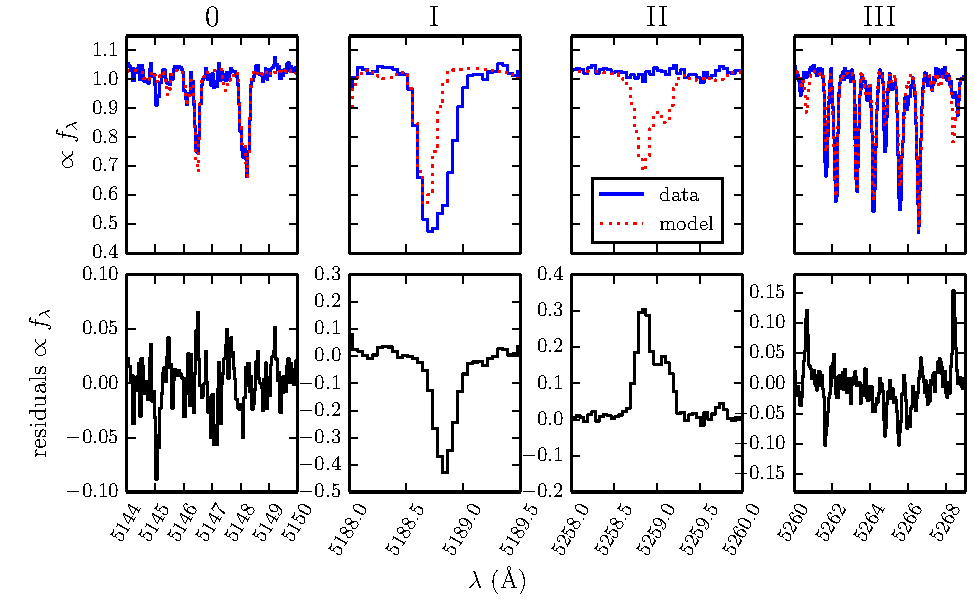
\includegraphics{figs/badlines.pdf}
\figcaption{A particularly illustrative spectral region with substantial localized structure in 
the residuals due to ``outlier" spectral lines in the model library.  For any specific line, there 
might exist a set of model parameters, $\vT$, that will improve its match with the data, but a 
$\vT$ that will properly fit \emph{all} the outlier lines does not exist in a pre-computed library 
with (necessarily) limited parametric flexibility.  Out of concern that such intrinsic mismatches 
can bias the inference on $\vT$, the methodology advocated here introduces local kernels to inflate 
the covariance around these outliers, self-consistently down-weighting their influence on the fit.  
\label{fig:badlines}}
\end{center}
\end{figure}

These local kernels can be modified to account for more complex residual structures.  For example, 
late-type stars with imperfectly modeled molecular bandheads may produce a complicated pattern of 
positive and negative residuals or a pronounced mismatch over a relatively large spectral scale.  
This phenomenologically different local covariance behavior can still be treated in this framework 
if an appropriate kernel morphology is adopted. 

\begin{figure*}[!htb]
\begin{center}
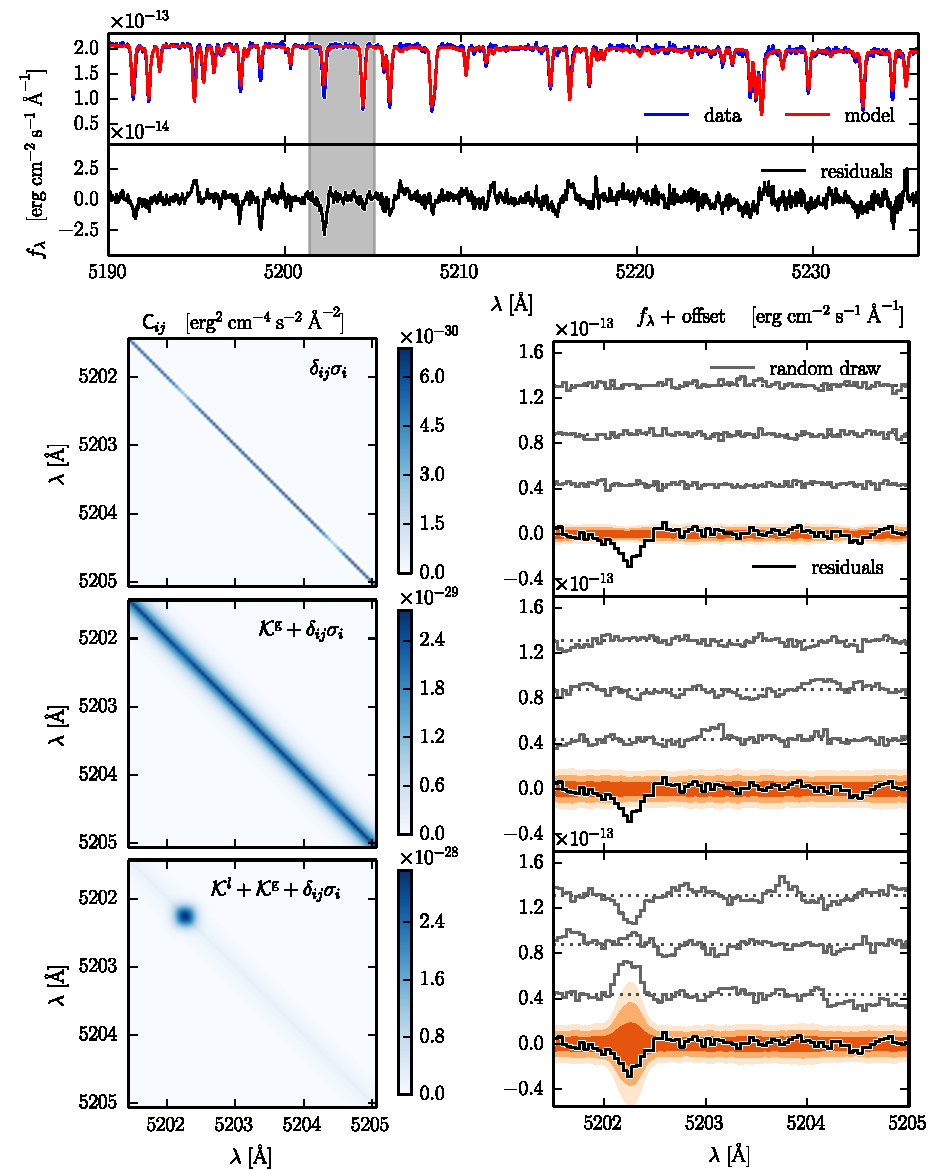
\includegraphics[scale=1.05]{figs/matrix_compilation.pdf}
\figcaption{A decomposition of the modeling procedure, explicitly highlighting the roles of the 
various contributions to the covariance matrix.  The top panels show a typical comparison between 
the data and model spectrum, along with the associated residual spectrum.  The subsequent panels 
focus on the illustrative region shaded in grey.  The left column of panels show the corresponding 
region of the covariance matrix $\vC$, decomposed into its primary contributions: from top to 
bottom, the trivial noise matrix, then combined with the global covariance kernel, and finally 
including an appropriate local covariance kernel.  In the right column, we show the zoomed-in 
residual spectrum ({\it black}) along with example random draws from the subsets of $\vC$ exhibited 
to the left.  The shaded contours ({\it orange}) represent the 1, 2, and 3\,$\sigma$ dispersions of 
an ensemble of 200 random draws from $\vC$.  Note that the trivial noise matrix ($\delta_{ij} 
\sigma_i$) poorly reproduces both the scale and structure of the residual spectrum.  The addition 
of a global kernel ($\mathcal{K}^{\rm g}$) more closely approximates the structure and amplitude of 
the residuals, but misses the outlier line at 5202.2\,\AA.  Including a local kernel 
($\mathcal{K}^l$) at that location results in a covariance structure that does an excellent job 
reproducing all the key residual features.  \label{fig:matrix}}
\end{center}
\end{figure*}


\subsubsection{Composite Covariance Matrix}

We can now compute the covariance matrix employed in the likelihood calculation 
(Eq.~\ref{eqn:lnlikelihood}) as the linear combination of the trivial pixel-by-pixel noise matrix 
and the global and local kernels discussed above,\footnote{See the Appendix for a modification of 
the likelihood function that incorporates interpolation uncertainty.} 
\begin{equation}
\vC_{ij}(\cov)  = b \, \delta_{ij} \, \sigma_i + w_{ij} \, \Kglobal_{ij}(\vp_{{\mathsf C}, g}) + 
                  \Klocal_{ij}(\vp_{{\mathsf C}, l}), 
\end{equation}
with (hyper-)parameters $\cov = [\vp_{{\mathsf C}, g}, \vp_{{\mathsf C}, l}]$.  The factor $b$ is 
a parameter that scales up the Poisson noise in each pixel by a constant factor to account for 
additional detector or data reduction uncertainties (e.g., read noise, uncertainties in the 
spectral extraction procedure, etc.); typically $b < 1.1$ for well-calibrated optical spectra.  If 
there are $N_{\rm loc}$ local covariance patches (see Section \ref{subsec:MCMC} on how this is 
determined), then there are $4N_{\rm loc}+2$ elements in the set of covariance (hyper-)parameters, 
$\cov$.  

Figure \ref{fig:matrix} provides a graphical illustration of how the kernels that comprise the 
covariance matrix are able to reproduce the structure present in a typical residual spectrum (for 
the sake of clarity, the interpolation error kernel is discussed separately, in the Appendix).  


\subsection{Priors} \label{subsec:priors}

The Bayesian framework of this inference approach permits us to specify prior knowledge about the 
model parameters, $p(\vM)$.  Since a high quality spectrum provides so much information about 
$\vT$, the inference of these parameters ends up not being very sensitive to the priors.  To be 
conservative, we generally recommend assigning uniform priors on $\vT$, such that $p(\vt_{\ast})$
is flat over the spectral library grid (and zero elsewhere) and $p(\vt_{\rm obs})$ is flat if 
$\vt_{\rm obs} \ge 0$ (i.e., for physically meaningful values).  

For (early type) stars with a clear continuum, it makes sense to assume flat priors on the 
polynomial parameters $\cheb$.  However, if information about the accuracy of the calibration is 
available (e.g., from observations of multiple spectrophotometric standards), it is possible to 
encode this information in a simple prior on the Chebyshev coefficients.  A reasonable example is a 
set of Gaussian priors with widths that encapsulate the systematic (fractional) variance of the 
derived calibration functions.  For (late type) stars with a poorly defined pseudo-continuum, 
some judicious tapering of the priors (such that high-$n$ coefficients are constrained around zero) 
may be required to ensure that broad spectroscopic features are not absorbed into the polynomial 
(see Section~\ref{sec:examples}). 

We suggest assuming uniform priors on the global kernel parameters.  For the local kernels, we 
typically adopt flat priors for the amplitudes and means \{$a_k$, $\mu_k$\}, but construct a 
specialized prior for the widths \{$\sigma_k$\} that is flat below the instrumental broadening 
width (when $\sigma_k < \sigma_v$) and has a rapid (logistic) taper to zero at larger values.  This 
form is designed to prevent the local kernels from diffusing to large $\sigma_k$ and low $a_k$,
since such behavior is better treated by the global kernel.  


\subsection{Exploring the Posterior} \label{subsec:MCMC}

The inference problem developed here has a natural hierarchical structure between the collections 
of ``interesting" parameters, $\vT = [\vt_{\ast}, \vt_{\rm obs}]$, and ``nuisance" hyperparameters, 
$\vP = [\cheb, \cov]$.  To explore the posterior distribution of the model conditioned on the data
\begin{equation} 
p(\vT, \vP | \vD) \propto p(\vD | \vT, \vP) \, p(\vT, \vP)
\label{eqn:post}
\end{equation}
for this type of structure, it is convenient to use MCMC simulations with a blocked Gibbs 
sampler coupled to the Metropolis-Hastings algorithm.  To summarize, this procedure works by 
sampling in a subset of parameters (with Metropolis-Hastings) conditioned on the current (fixed) 
values of the other parameters; after each iteration, the Gibbs sampler then updates the values of 
the sampled parameter subset and then cycles through all the (previously fixed) different parameter 
subsets in the same way (for a more nuanced mathematical description of the process, see Chapter 11 
of \citealt{gelman13}).  A step-by-step prescription follows, where the $i^{\rm th}$ 
iteration of the Gibbs sampler is indexed with a superscript: \\

\noindent (1) Initialize the parameters.  One might set $\vT^0$ based on estimates in the 
literature or scaling behaviors, and make simple assumptions about $\vP^0$.  Here, we set the 
Chebyshev coefficients ($\cheb^0$) so that the polynomials are constant ($c_o^{(0)} = 1$,  
$c_o^{(>0)} = 0$, $\forall$ $o$) and assume only the trivial noise spectrum and interpolation error 
kernel contribute to the covariance matrix ($\cov^0 = 0$).  \\

\noindent (2) Start the $i^{\rm th}$ (where $i \in [1,N_G]$) iteration of the Gibbs sampler.  For 
each iteration of the Metropolis-Hastings algorithm, sample in the interesting parameters $\vT$ to 
evaluate the posterior (Eq.~\ref{eqn:post}) following the framework laid out in Sections 
\ref{subsec:likelihood} and \ref{subsec:priors}.  This represents a ``slice" through the posterior 
space conditioned on the nuisance parameters being held fixed ($\vP = \vP^{i-1}$).  Then update the 
interesting parameters $\vT^{i-1} \rightarrow \vT^i$. \\

\noindent (3) Cycle through and update the nuisance parameters, $\vP^{i-1} \rightarrow \vP^i$.  For 
each spectral order,   

\begin{enumerate}[(a)]
\item Sample in the polynomial coefficients $\cheb$ along a subset of the posterior space where 
$\vT^i$ and $\cov^{i-1}$ are fixed.  Update the coefficients, $\cheb^{i-1} \rightarrow \cheb^i$.  

\item Sample in the global (stationary) kernel parameters, $\vp_{{\mathsf C},g} = [a_g, \ell]$, 
with $\vT^i$, $\cheb^i$, and the local kernel parameters, $\vp_{{\mathsf C}, l}^{i-1}$, fixed.  
Update $\vp_{{\mathsf C}, g}^{i-1} \rightarrow \vp_{{\mathsf C}, g}^i$.

\item If any local (non-stationary) kernels have been instantiated (see below), sample in their 
hyperparameters $\vp_{{\mathsf C},l}$ with $\vT^i$, $\cheb^i$, and $\vp_{{\mathsf C}, g}^i$ fixed.  
Update the local kernel parameters $\vp_{{\mathsf C}, k}^{i-1} \rightarrow \vp_{{\mathsf C}, k}^i$. 

\end{enumerate}

\noindent (4) Return to Step~(2) and iterate.  After a burn-in period, periodically pause the Gibbs 
sampler and compute the Gelman-Rubin convergence diagnostic, $\hat{R}$ \citep[][their 
Eq.~11.4]{gelman13}.  Break the loop if $\hat{R} \, < \, 1.1$.  \\

\noindent (5) Repeat the procedure in Steps~(1)--(4) with different initializations and compute 
convergence diagnostics to ensure that all of the chains have reached the same global maximum in 
the posterior probability distribution. \\

In Step~(3c), local covariance kernels are instantiated into the model according to the following 
procedure.  First, an ``average" residual spectrum is generated by combining $\sim$500 residual 
spectra that were stored during a burn-in period using only the global kernels (prior to this 
storage, the Markov chain is thinned to account for autocorrelation of the posterior samples).  
This average spectrum is then iteratively examined for deviations outside a critical threshold; 
when a large residual is identified, a local kernel is introduced with a mean ($\mu_k$) at its 
location.\footnote{Although this may seem similar to the procedure of ``sigma-clipping", there is a 
crucial difference.  Rather than rejecting outlier data once it is found (i.e., setting its weight 
in the inference problem to zero), this procedure will actually self-consistently determine how to 
weight the outliers inside the probabilistic framework.}  After some experimentation with different 
threshold levels, we have adopted a criterion whereby a kernel is instantiated where the local 
residual is at least 4$\times$ the standard deviation in the average residual 
spectrum.\footnote{Lower thresholds result in more local kernels, thereby reducing the amplitude of 
the global kernel.  In the extreme case of a very low threshold, a local kernel would be 
instantiated for every spectral line (and no global kernel would be required).  We found that 
ultimately the posterior inferences on the parameters of interest are relatively insensitive to the 
choice of a threshold level, so long as it is set low enough to capture the egregious outliers.}  
Alternative instantiation schemes, such as re-evaluating the locations of kernels with each 
iteration of the Gibbs sampler, yield similar results; however, the adopted approach was found to 
consistently converge with minimal computational overhead.  Once all of the necessary local kernels 
have been instantiated, the Gibbs sampler is run for another period of burn-in.\footnote{There is 
no practical reason to delete local kernels once instantiated.  If the parameters have changed such 
that a given local kernel is no longer required, that kernel amplitude will be driven towards zero 
and represent a negligible contribution to $\vC$; in effect, the model will act as if the kernel 
were deleted automatically.}

This procedure can be a significant computational challenge.  A typical data spectrum has $N_{\rm 
pix} > \mathcal{O}(10^3)$, and therefore the many evaluations of the matrix product $\vR^{\trans} 
\vC^{-1} \vR$ in the likelihood calculation can be numerically expensive.  However, because $\vC$ 
is a symmetric, positive semi-definite matrix, we can employ Cholesky factorization to optimize the 
evaluation of the matrix product and avoid the direct calculation of the matrix inversion 
($\vC^{-1}$).  For multi-order echelle spectra or multiple spectra of the same target (perhaps 
taken with different instruments), the nuisance parameters for each segment of the spectrum are 
independent. This means that the computationally intensive steps of generating a model spectrum
for a specific wavelength range and evaluating the likelihood can be parallelized. The only segment 
of the code that needs to be synchronized is the MCMC proposal of stellar parameters, which are 
shared between all chunks of the spectrum.  The massive parallelization of this algorithm on a 
computer cluster therefore enables the simultaneous inference of interesting parameters over wide 
spectral ranges at high resolution, or from multiple datasets.  To sample the posteriors in this 
mode, we extend the Metropolis-Hastings sampler included in the {\tt emcee} package 
\citep{foreman-mackey13} to function within a parallelized blocked Gibbs 
sampler.\footnote{See \url{https://github.com/iancze/emcee}.}\\


\section{Demonstrations} \label{sec:examples}

In this section, we aim to demonstrate the functionality and highlight the flexibility and utility 
of the probabilistic inference methodology described above.  To do that, we illustrate how the 
modeling framework operates for two representative examples.  The first is an elaboration of the 
example shown throughout Section \ref{sec:method}, using a high resolution optical 
($\sim$5000-5400\,\AA) spectrum of the F5 dwarf main sequence star (and transiting exoplanet host) 
WASP-14 \citep{joshi09,torres12}.  This spectrum is interpreted in the context of two different 
synthetic model libraries: a custom modification of the \citet{castelli04} models designed and 
empirically calibrated to reproduce well the optical spectrum around the \ion{Mg}{1}\,b triplet at 
$\sim$5100\,\AA\ for Sun-like stars (used in {\tt SPC}; hereafter the {\sc CfA/Kurucz} library), 
and the most recent incarnation of the {\sc Phoenix} library \citep{husser13}.  The second 
example uses a medium resolution near-infrared ($\sim$2.0-2.4\,$\mu$m) spectrum of the M5 dwarf 
star Gliese\,51 (hereafter Gl\,51), observed as part of the NASA/IRTF library of spectral standards 
\citep{cushing05,rayner09}.  In this case we use the {\sc Phoenix} library to generate models, 
since it is well-sampled at cooler temperatures.


\subsection{WASP-14} \label{subsec:wasp}

A high resolution ($R\approx44,000$) optical spectrum of WASP-14 was obtained on 2009 June 14 
using the Tillinghast Reflector Echelle Spectrograph \citep[TRES;][]{furesz08} on the Fred Lawrence 
Whipple Observatory 1.5\,m telescope.  TRES delivers an echelle spectrum with 51 orders that cover 
the optical range from 3860--9100\,\AA.  The data were reduced and calibrated using standard 
techniques in the TRES pipeline (cf.,~\citealt{buchhave10}; see \citealt{torres12} for more 
specific details).  At 5100\,\AA, the S/N is $\sim$150 per resolution element.  

\citet{torres12} originally acquired these data in an effort to measure the WASP-14 stellar 
properties, and thereby better constrain the parameters of the transiting exoplanet it hosts.  To 
that end, they employed the {\tt MOOG} and {\tt SPC} approaches outlined in Section 
\ref{sec:intro}.  Their analysis was performed in two ways, with the surface gravity treated as a 
free parameter or assumed to be fixed (to $\log g = 4.29$) based on an inference of the mean 
stellar density from the exoplanet transit depth and a comparison of WASP-14 photometry to stellar 
evolution models in the H-R diagram \citep{joshi09}.  Only parameter inferences from the latter 
assumption were reported.  The {\tt MOOG} analysis employed \citet{kurucz93} atmospheres to 
synthesize a suite of individual \ion{Fe}{1} and \ion{Fe}{2} lines in the $\sim$4300--6750\AA\ 
region, whose equivalent widths were compared with the TRES measurements in a simple least-squares 
sense.  This approach suggests that $T_{\rm eff} = 6150\pm75$\,K and $[{\rm Fe/H}] = 
-0.34\pm0.10$\,dex.  The {\tt SPC} analysis relied on a direct comparison between three TRES 
spectral orders covering $\sim$5100-5400\,\AA\ and synthetic spectra from the {\sc CfA/Kurucz} 
library; it indicates $T_{\rm eff} = 6507\pm50$\,K, $[{\rm Fe/H}] = -0.15\pm0.08$\,dex, and $v \sin 
i = 3.9\pm0.5$\,km s$^{-1}$.  The uncertainties are dominated by a ``floor" contribution, imposed 
independently on each parameter and meant to be representative of the systematics (a standard 
procedure in this field).  

Given the decision to employ a spectral library to generate models (Sect.~\ref{subsec:synthetic}), 
a direct comparison of the \citeauthor{torres12}~{\tt SPC} result with our framework is most 
relevant.  Using the same TRES spectral orders, the {\sc CfA/Kurucz} library, and a 
$\delta$-function prior on $\log g$ (at 4.29), we infer parameters that are roughly consistent with 
the {\tt SPC} approach; see Table~\ref{table:Kurucz}.  Figure~\ref{fig:Kurucz_residuals} 
demonstrates the quality of our approach in reproducing the WASP-14 spectrum and, especially 
significant, the structure of the residuals.  Figure~\ref{fig:Kurucz_posterior} shows marginal 
projections of the posterior-space, highlighting key parameter degeneracies.  

\begin{figure*}[!t]
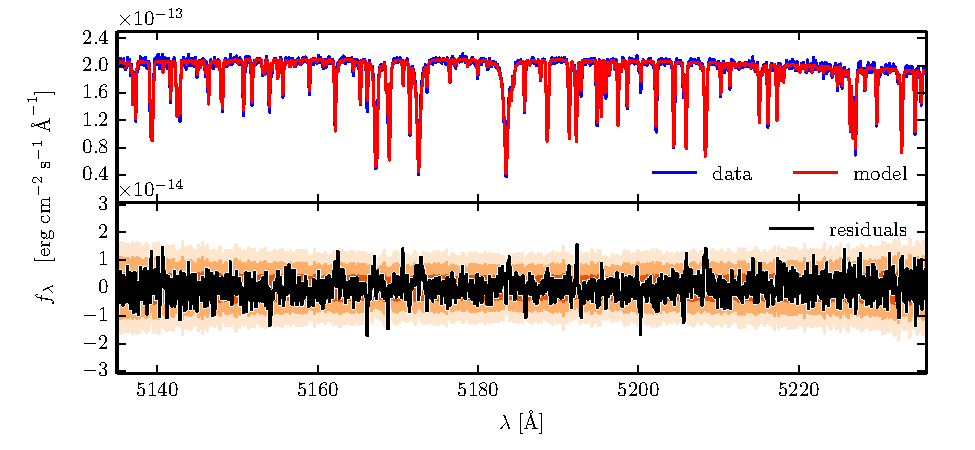
\includegraphics{figs/residuals_Kurucz_logg.pdf}
\vspace{-0.3cm}
\figcaption{({\it top}) A representative segment of the TRES spectrum of WASP-14 ({\it blue}), 
overlaid with a {\sc CfA/Kurucz} model ({\it red}) generated by drawing parameters from the 
posterior distribution (for a fixed $\log g = 4.29$).  ({\it bottom}) The residual spectrum along 
with contours representing the distributions of a large number of random draws from the covariance 
matrix (the shading is representative of the 1, 2, and 3\,$\sigma$ spreads of that distribution of 
draws), as in Fig.~\ref{fig:matrix}.  With such a finely tuned model library, local covariance 
kernels are not required.  \label{fig:Kurucz_residuals}}
\vspace{0.2cm}
\end{figure*}

\capstartfalse
\begin{deluxetable}{lr@{ $\pm$ }l|r@{ $\pm$ }l}[!b]
\tablecaption{\label{table:Kurucz}Inferred Parameters for WASP-14}
\tablehead{\colhead{Parameter} & \multicolumn{2}{c}{{\sc CfA/Kurucz}} & \multicolumn{2}{c}{{\sc Phoenix}}}
\startdata
$T_{\rm eff}$ (K) & 6424     & 19                      &  6354   & 39        \\
$\log g$      & 4.29     & 0 (fixed)               &  4.29   & 0 (fixed) \\
$\Z$          & -0.26    & 0.01                    & -0.30  & 0.02     \\
$v \sin i$ ($\kms$)\tablenotemark{a}   & 4.47 & 0.06       &  5.09   & 0.06      \\
$v_z$ ($\kms$)        & -4.60    & 0.02                    & -4.86   & 0.02      \\
$\log \Omega$\tablenotemark{b} & -12.7180 & 0.0004 & -12.717 & 0.0007 \\
$A_V$                          & 0        & 0 (fixed) & 0 & 0 (fixed)
\enddata
\tablenotetext{a}{Small differences in the rotational broadening between the two libraries are
expected, since they assume different micro- and macro-turbulence behavior in the stellar
atmospheres.}
\tablenotetext{b}{For the spectral emulator (Appendix~\ref{sec:Appendix}), the models are scaled to 
an average flux of unity, rather than flux at the stellar surface; the quoted values are unknown 
multiples of $R^2/d^2$.}
\tablecomments{The quoted values represent the ``best-fit", the peak of the marginal posterior 
distributions for each parameter.  The quoted uncertainties correspond to the 68.3\%\ 
($\sim$1\,$\sigma$) confidence intervals.  Expanded lists of the inferred values and uncertainties 
for all nuisance parameters are available electronically.}
\end{deluxetable}
\capstarttrue

\begin{figure}[!b]
  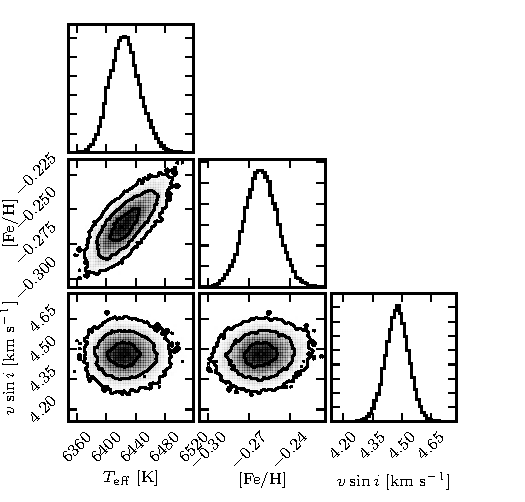
\includegraphics{figs/Kurucz_triangle.pdf}
\vspace{-0.5cm}
  \figcaption{The posterior probability distributions for the interesting stellar parameters 
(marginalized over all other model parameters) of WASP-14 based on the {\sc CfA/Kurucz} model 
library, as explored by the MCMC Gibbs sampler.  For the two-dimensional posterior projections, 
contours are drawn at the standard 1, 2, and 3\,$\sigma$ levels (of a normal distribution) for 
reference.  \label{fig:Kurucz_posterior} }
\end{figure}

It is worthwhile to comment on the inferred parameter uncertainties.  In this specific example, 
some experimentation with restricted forms of the covariance matrix confirms that the uncertainties 
of the interesting parameters have roughly equal contributions from trivial (Poisson) noise, grid 
interpolation errors, and a non-trivial global covariance term.\footnote{Note that the {\sc 
CfA/Kurucz} library has been specifically well-tuned for stars like WASP-14, by careful variation 
of atomic data (e.g., line lists, oscillator strengths) with reference to observations of the Sun 
and Vega, by J.~Morse and J.~B.~Laird.  Over this limited spectral range, this means that no local 
covariance kernels need to be instantiated to reproduce the residual structure.}  For synthetic 
models that are less well-tuned than the {\sc CfA/Kurucz} grid, the latter two terms will certainly 
dominate.  In any case, these uncertainties are still considerably smaller than the ``floor" values 
imposed by \citet{torres12}, but they are representative of our expectations for comparing data of 
high sensitivity and volume with models of limited parametric flexibility (i.e., the uncertainties 
would inflate considerably if the many fixed or restricted parameters that went into building the 
model libraries were available for variation).  

\begin{figure*}[!htb]
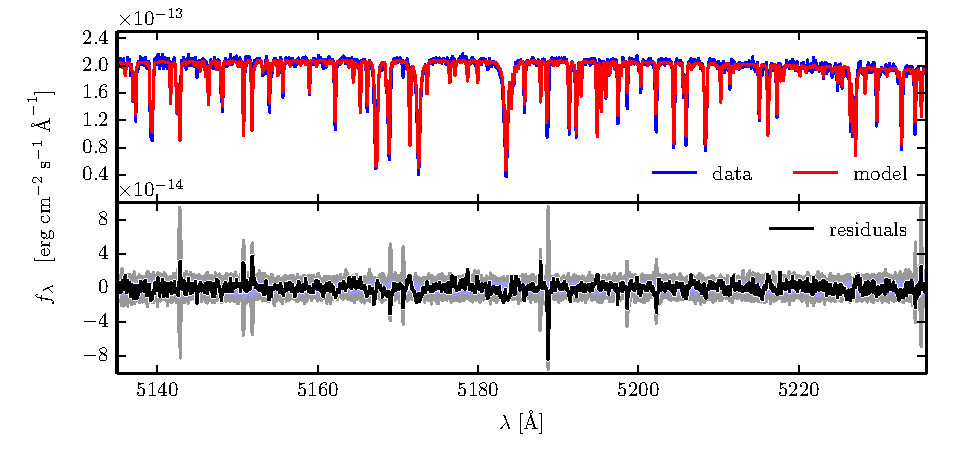
\includegraphics{figs/residuals_PHOENIX_logg.pdf}
\vspace{-0.3cm}
\figcaption{Same as Fig.~\ref{fig:Kurucz_residuals} for the {\sc Phoenix} models.  Note the
increased vertical scale and local covariance structure for the residuals.  
\label{fig:PHOENIX_residuals}}
\vspace{0.2cm}
\end{figure*}

\begin{figure}[!b]
\begin{center}
  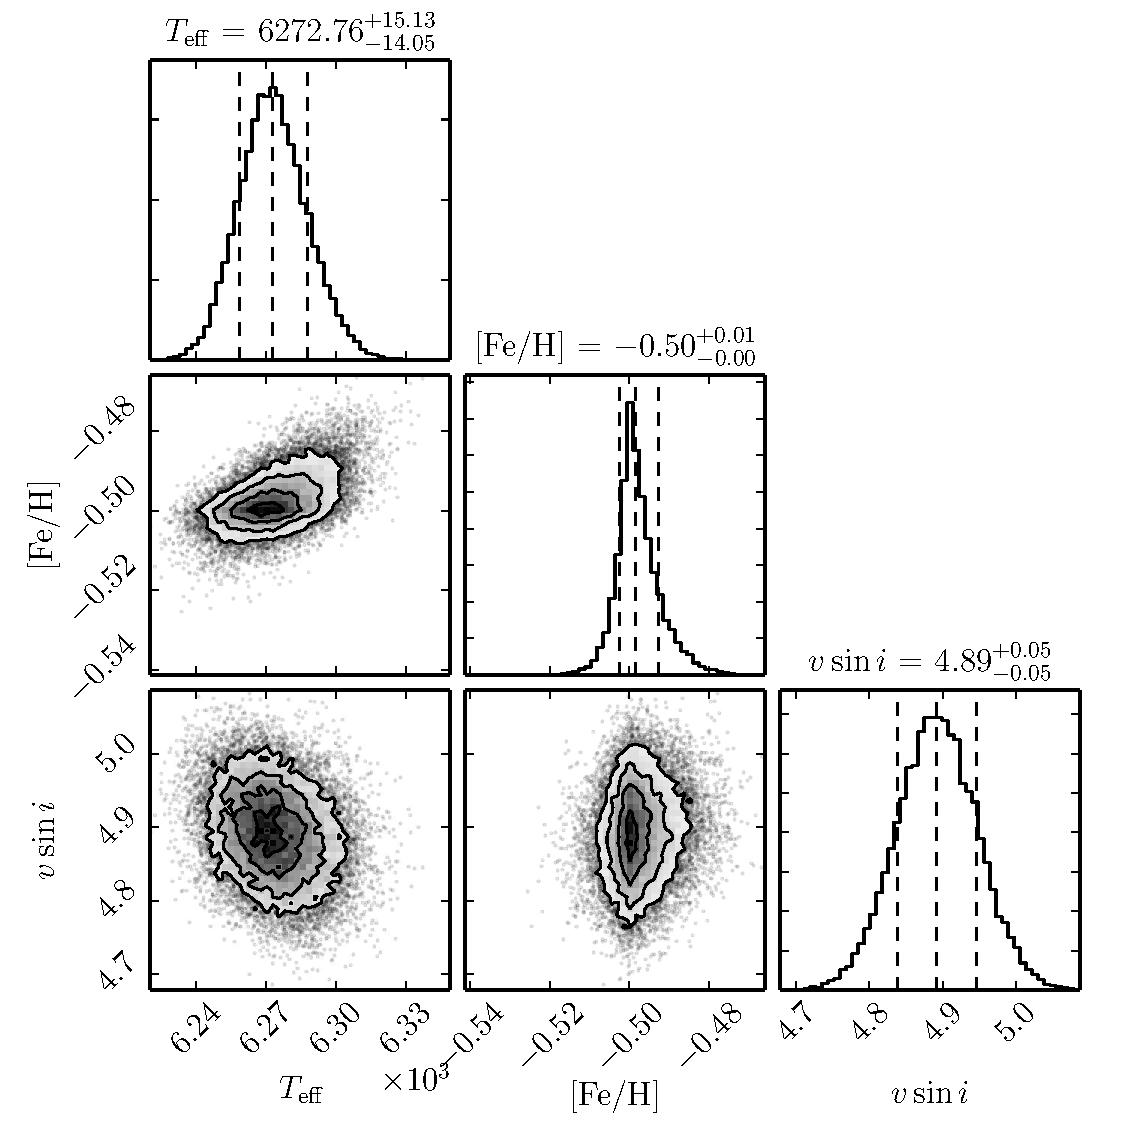
\includegraphics[width=0.5\textwidth]{figs/PHOENIX_triangle.pdf}
\vspace{-0.5cm}
\figcaption{Same as Fig.~\ref{fig:Kurucz_posterior}, but for the {\sc Phoenix} models.
\label{fig:PHOENIX_posterior}}
\end{center}
\end{figure}

There are two additional, {\it systematic} sources of uncertainty that merit attention.  First are 
those associated with the instrument and/or calibration procedure.  Common practice is to quantify 
these contributions by comparing parameter inferences made using different spectra (e.g., from 
different instruments or observing nights): the results are usually presented as an average, with 
uncertainties inflated by adding in quadrature parameter-independent terms that account for the 
dispersion between the inferences from individual spectra.  To quantify these instrumental 
systematics for WASP-14, we modeled three other TRES spectra obtained by \citet{torres12} 
independently (under the same assumptions).  We found a scatter of $\sim$20\,K in $T_{\rm eff}$ and 
$\sim$0.02\,dex in $\Z$ between the individual inferences, a testament to quality calibration and 
an exceptionally stable spectrograph.  The more appropriate way of combining the inferences is to 
model these four spectra simultaneously in our hierarchical framework: we found that the parameter 
inferences become slightly more precise (as would be expected for a weighted average and well-tuned 
models), while preserving the intrinsic parameter degeneracies (which is not possible in the 
weighted average approach).

A second source of systematic uncertainty lies with the models themselves, including the treatment 
of structure, assumptions about boundary conditions (convection, etc.), and the employment of 
fundamental atomic and molecular data.  As a benchmark for estimating the scope of this kind of 
uncertainty, we repeated the analysis described above using instead the {\sc Phoenix} model 
library.  Because the {\sc Phoenix} model spectra cover a much broader spectral range that has not 
been fine-tuned for solar type stars (unlike the {\sc CfA/Kurucz} library), this has the added 
benefit of demonstrating a key feature of the modeling framework -- the treatment of spectral line 
``outliers" with local patches of high covariance (Sect.~\ref{subsec:local_covariance}) in a 
sophisticated likelihood function.  

Figure~\ref{fig:PHOENIX_residuals} illustrates the approach in practice through a comparison of the 
WASP-14 data and the {\sc Phoenix} models.  There are two notable differences in the residual 
spectra presented there and in the corresponding Figure~\ref{fig:Kurucz_residuals} for the {\sc 
CfA/Kurucz} models.  First, the amplitude of the global covariance structure is twice as large for 
the {\sc Phoenix} models: since that amplitude is an indirect parameterization of the {\it fit 
quality}, this indicates that the {\sc Phoenix} models present an overall worse match to the 
data.  Second, there are several local regions of strong residuals (outlier lines), which are 
enveloped in a parametric treatment of the local covariance structure.  In effect, we have modeled 
the large residuals with a suite of individual covariance kernels, with parameters that identify 
and appropriately down-weight imperfect model spectral lines in a self-consistent manner.

Aside from the structure of the covariance matrix, there is also a modest difference between the 
posterior distributions of the stellar parameters inferred using the {\sc Phoenix} and {\sc 
CfA/Kurucz} libraries: see Table~\ref{table:Kurucz} and compare Figures~\ref{fig:Kurucz_posterior} 
and \ref{fig:PHOENIX_posterior}.  The {\sc Phoenix} models find a systematically cooler temperature 
(by $\sim$75\,K) and lower metallicity than the {\sc CfA/Kurucz} models.  Because our framework 
explicitly mitigates the potential for posterior bias from imperfect matches between data and 
models, these apparent discrepancies must be intrinsic to the different input physics of the model 
libraries.\footnote{It is worth noting that these differences are not a manifestation of the 
stringent prior on surface gravity.  When the spectra are modeled with $\log g$ unconstrained, the 
posteriors for both libraries shift, but their respective discrepancies actually increase 
slightly.}  Such a comparison serves as a stark reminder that incomplete and/or over-simplified 
physical prescriptions remain the most significant source of systematic uncertainty in estimates of 
fundamental stellar parameters.

\begin{figure*}[!htb]
  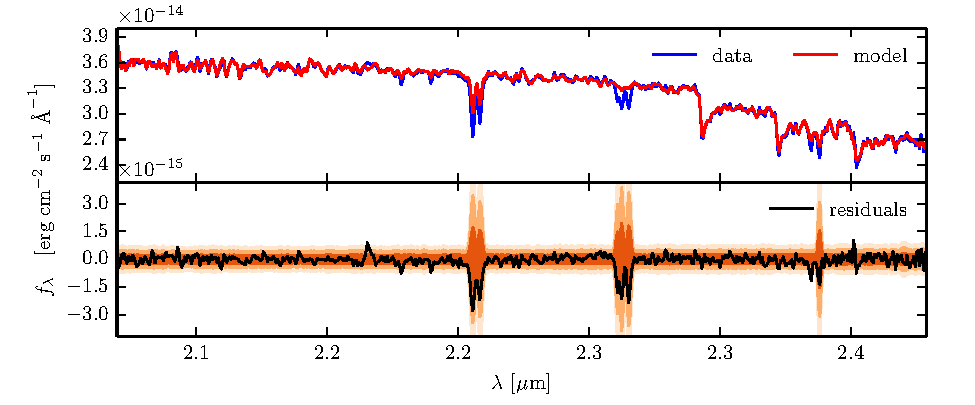
\includegraphics{figs/residuals_Gl51_logg.pdf}
\vspace{-0.3cm}
  \figcaption{The $K$-band SPEX spectrum of Gl~51 ({\it blue}) compared with a
  {\sc Phoenix} model ({\it red}) generated by drawing parameters from the
  posterior distribution. ({\it bottom}) The residual spectrum along with
  contours representing the distributions of a large number of random draws
  from the covariance matrix (the shading is representative of the 1,
2, and 3\,$\sigma$ spreads of that distribution of draws), as in Fig.~\ref{fig:Kurucz_residuals}.  
Note how the ``outlier" features are clearly identified and treated by the local covariance kernels.
\label{fig:Gl51_residuals}}
\vspace{0.2cm}
\end{figure*}

\begin{figure}[!b]
  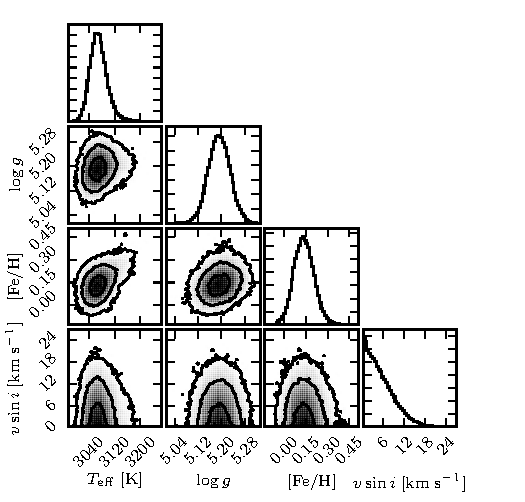
\includegraphics[width=0.5\textwidth]{figs/Gl51_triangle.pdf}
  \figcaption{The posterior probability distributions for the interesting stellar parameters
(marginalized over all other model parameters) of Gl~51 based on the {\sc Phoenix} model library,
as explored by the MCMC Gibbs sampler.  For the two-dimensional posterior projections, contours are
drawn at the standard 1, 2, and 3\,$\sigma$ levels (of a normal distribution) for reference.
\label{fig:Gl51_posterior}}
\end{figure}

\subsection{Gl~51}

A moderate resolution ($R\approx2,000$) near-infrared spectrum of Gl~51 was obtained on 2000 
Nov 6 using the SPEX instrument \citep{rayner03} on the 2.3\,m NASA Infrared Telescope Facility 
(IRTF).  SPEX is a cross-dispersed echelle spectrograph that covers the red-optical to 
thermal-infrared spectrum (0.7--5.5\,$\mu$m) in two settings.  These data were obtained as part of 
the IRTF spectral standard library project \citep{cushing05,rayner09}, and were processed through 
the well-vetted {\tt Spextool} reduction pipeline \citep{cushing04,vacca03} to deliver a fully 
calibrated spectrum.  At 2.1\,$\mu$m, the S/N is $\sim$400 per resolution element.

Modeling late-type stellar atmosphere structures and their spectra is considerably more complex 
than for Sun-like stars, due to lingering uncertainties in the atmosphere physics and molecular 
opacities.  Especially confounding is the presence of complex condensates (clouds) at the coolest 
temperatures \citep{allard13}, making it considerably more challenging to determine (sub-)stellar 
properties \citep{rajpurohit14}.  Various approaches have been taken to infer the key parameters in 
the face of these difficulties, including iteratively masking regions with poor spectral agreement 
\citep[e.g.,][]{mann13}.  Astutely, \citeauthor{mann13}~note that such a scheme may exclude 
regions of the spectrum that contain intrinsically useful information for discriminating between 
physical properties, and that a more sophisticated approach would weight each spectral region based 
on its consistency with the data.  The modeling framework that we have constructed here does 
exactly that.

As a point of reference, \citet{rojas-ayala12} used a $K$-band spectrum at similar resolution to 
the SPEX data to estimate the basic Gl~51 parameters using an indexing technique.  They measured 
equivalent widths for the 2.205\,$\mu$m \ion{Na}{1} doublet and 2.263\,$\mu$m \ion{Ca}{1} triplet, 
along with a pseudo-continuum index defined over three narrow passbands, 2.070--2.090, 
2.235--2.255, and 2.360--2.380\,$\mu$m (see their Fig.~2 for a useful visualization), designed to 
probe the spectral curvature induced by H$_2$O absorption bands.  With reference to a custom grid 
of the {\sc BT-Settl} modifications of the {\sc Phoenix} library \citep{allard12}, 
\citeauthor{rojas-ayala12}~infer $T_{\rm eff} = 3039\pm56$\,K and $[{\rm Fe/H}] = 0.28\pm0.17$ for 
a fixed $\log g = 5.0$.  

By modeling the $K$-band region of the SPEX data with the {\sc Phoenix} library\footnote{The 
differences between the \citet{husser13} {\sc Phoenix} library and the {\sc BT-Settl} modification 
of the {\sc Phoenix} models at these (relatively) high effective temperatures are minor.  Since the 
former is defined over a well-sampled, more regular grid of stellar parameters, we prefer it here 
for computational simplicity.} and a Gaussian prior on $\log g$ (at $5.0 \pm 0.05$ dex), we infer 
parameters for Gl~51 that are consistent with \citet{rojas-ayala12}.  
Figure~\ref{fig:Gl51_residuals} displays the spectral modeling results, and 
Figure~\ref{fig:Gl51_posterior} shows the marginal posterior distributions for the relevant stellar 
parameters.  The best-fit parameter values and their associated uncertainties are compiled in 
Table~\ref{table:Gl51}.

We concur with \citet{rojas-ayala12} that the {\sc Phoenix} models manage to match the overall 
spectral morphology of mid-M type stars well, but consistently under-predict the strengths of the 
\ion{Na}{1} and \ion{Ca}{1} resonance lines, even for high metallicities.  \citet{rajpurohit10} 
speculated that this discrepancy may be a consequence of inaccurate atomic data (oscillator 
strengths and/or opacities).  Our approach uses local covariance kernels to self-consistently 
determine the ``weights" of discrepant spectral lines in the overall fit.  In that sense, these 
outlier features still bring their full information content to bear on the posterior distributions 
of the stellar parameters without imposing a systematic bias.  Figure~\ref{fig:Gl51_residuals} 
demonstrates that these features have been identified as problematic, resulting in localized 
patches of appropriately inflated covariance.

\capstartfalse
\begin{deluxetable}{lr@{ $\pm$ }l}[h]
\tablecaption{\label{table:Gl51}Inferred Parameters for Gl 51}
\tablehead{\colhead{Parameter} & \multicolumn{2}{c}{{\sc Phoenix}}}
\startdata
$T_{\rm eff}$ (K) & 3071  & 28 \\
$\log g$ & 5.19 & 0.04 \\
$\Z$ & 0.14 & 0.07 \\
$v \sin i$ ($\kms$) & \multicolumn{2}{c}{$\leq 15.0$} \\
$v_z$ ($\kms$) & 11.6 & 1.3 \\
$\log \Omega$ (sr) & -13.481  & 0.001 \\
$A_V$ & 0 & 0 (fixed)
\enddata
\tablecomments{Notation as in Table~\ref{table:Kurucz}.}
\end{deluxetable}
\capstarttrue

The fitting methodology adopted here could prove especially useful in spectroscopic inference for
cool stars like Gl~51, where substantial uncertainties in their more complex atmospheres will 
naturally produce systematic deviations between models and data.  However, many of 
those discrepancies will be manifested in molecular features, which likely result in considerably 
more complex residual structures than noted here \citep[e.g., the TiO bands in the red-optical; 
see][their Fig.~9]{mann13}.  The overall framework we have employed should still function, although 
more appropriate local covariance kernels may need to be developed to capture the different nature 
of these outliers.  For example, one might employ hybrid kernels (like the product of a truncated 
exponential and a \matern\ kernel) or empirically-motivated parametric shapes (e.g., a saw-tooth 
pattern) to provide a better representation than a simple Gaussian feature.  \\



\section{Discussion} \label{sec:discussion}

Astronomers exploit spectroscopy to retrieve physical information about their targets.  Ideally, 
such inferences are made with the maximal precision afforded by the measurement noise, and do not 
suffer from any systematic bias.  But in practice, the spectral models used as references are never 
perfect representations.  Even modest mismatches between data and model can propagate substantial 
systematic uncertainty into the inference problem.  In high-sensitivity applications (e.g., stellar 
and exoplanetary astrophysics), ignoring these systematics can give a false sense of both precision 
and accuracy in the inferences of key parameters.  Typically, the more egregious of these 
imperfections are ``mitigated" by dismissal (explicitly not considering a subset of the data; e.g., 
masking, clipping).  Rarely, they are confronted directly with painstaking, computationally 
expensive fine-tuning of more general (nuisance) parameters in the model (e.g., oscillator 
strengths, opacities), albeit only over a very limited spectral range and region of physical 
parameter-space (e.g., the {\sc CfA/Kurucz} library; Sect.~\ref{subsec:wasp}).

We have presented an alternative approach to dealing with this fundamental issue, grounded in a 
generative, hierarchical Bayesian framework.  The method advocated here constructs a sophisticated 
likelihood function, employing a non-trivial covariance matrix to treat the correlated 
pixel-to-pixel residuals generated from intrinsically imperfect models.  That matrix is composed of 
a linear combination of {\it global} (stationary) and {\it local} (non-stationary) Gaussian 
process kernels, which parameterize an overall mild covariance structure as well as small patches 
of highly discrepant outlier features.  The approach we describe is generally applicable to any 
spectroscopic inference problem (e.g., population synthesis in unresolved star clusters or 
galaxies, physical/chemical models of emission line spectra in star-forming regions, etc.).  
Moreover, it has the flexibility to incorporate additional information (as priors) or parametric 
complexity (if desired), and could be deployed as a substitute for a simplistic $\chi^2$ metric in 
already-established fitting tools (e.g., {\tt SME}).  To demonstrate how it is used, we determined 
the surface parameters of main-sequence stars with mid-F and mid-M spectral types from high-S/N 
optical and near-infrared data, with reference to pre-computed model libraries 
(Sect.~\ref{sec:examples}).  The source code developed here is open and freely available for use: 
see \url{http://github.com/iancze/Starfish}.

The novelty of employing this kind of likelihood function in the spectroscopic inference problem is 
that the treatment of data--model mismatches (in essence, the fit quality) is explicitly built into 
the forward-modeling framework.  This offers the unique advantage that discrepant spectral features 
(outliers), which may contain substantial (even crucial) information about the parameters of 
interest, can still effectively propagate their useful information content into the posteriors with 
a weighting that is determined self-consistently.  From a practical standpoint, this means that 
{\it all of the data} can be employed in the inference problem without undue concern that the 
posteriors will be biased by model imperfections, even in the case of models with limited 
parametric flexibility (e.g., pre-computed spectral libraries).

Ultimately, the benefits of employing covariance kernels to accommodate imperfect models could 
be extended well beyond modeling the spectra of individual targets.  In principle, the approach we 
have described here can be used to systematically discover and quantify imperfections in spectral 
models and eventually to build data-driven improvements of those models that are more appropriate 
for spectroscopic inference.  Consider the specific application to stellar spectroscopy, which has 
been the focus here.  By fitting many stellar spectra with the same family of models, we can 
catalog the covariant structure of the fit residuals -- especially the parameters of the local 
covariance kernels -- to collate quantitative information about where and how the models tend to 
deviate from observational reality.  That information can be passed to the spectral synthesis 
community, in some cases enabling modifications that will improve the quality of the spectral 
models.  On a large enough scale, this feedback between observers and modelers could be used to 
refine inputs like atomic and molecular data (oscillator strengths, opacities), elemental abundance 
patterns, and perhaps the stellar atmosphere structures.

Alternatively, this kind of feedback could be used to make data-driven modifications to the already 
existing models, creating a new library of semi-empirical spectral models.  This could be 
accomplished by linking the parameters of the covariance kernels derived from fitting many spectra 
in a hierarchical Bayesian model, which would add confidence to the assessment that certain 
spectral features are {\it systematic} outliers and offer general quantitative guidance on how to 
weight them in the likelihood calculation.  Rather than simply assembling an empirical spectral 
library using only observations, this combined machine-learning approach would naturally provide a 
physical anchoring for the key physical parameters, since they are reflected in the spectra based 
on the physical assumptions in the original models.  This kind of large-scale analysis holds great 
promise in the (ongoing) era of large, homogeneous high resolution spectroscopic datasets (e.g., 
like those being collected in programs like the APOGEE and HERMES surveys; \citealt{nidever12,
zucker12}), since they provide enormous leverage for identifying and improving the underlying model 
systematics. \\

\acknowledgments  The authors would like to acknowledge the following people for many 
extraordinarily helpful discussions and key insights: Gregory M.~Green, Kaisey Mandel, Daniel 
Foreman-Mackey, John Johnson and the ExoLab, Daniel Eisenstein, Rebekah Dawson, Tom Loredo and the 
ExoStat group, Allyson Bieryla, and Maxwell Moe.  IC was supported by the NSF Graduate Fellowship 
and the Smithsonian Institution.  Figures \ref{fig:Kurucz_posterior}, \ref{fig:PHOENIX_posterior}, 
and \ref{fig:Gl51_posterior} were generated with \texttt{triangle.py} \citep{foreman-mackey14}.  
This research made extensive use of Astropy \citep{astropy13} and the Julia programming language 
\citep{julia12}.


\appendix

\section{Spectral Emulator for Interpolation} \label{sec:Appendix}

Interpolation from a library of synthetic spectra is conceptually straightforward, but in the 
application being considered here there are some subtleties that necessitate a more sophisticated 
approach.  Spectral line formation is a non-linear process, where line shapes are determined by 
complex radiative transfer through a stellar atmosphere.  Any interpolation process aims to bypass 
this non-linear process and predict the behavior of many different spectral lines for an arbitrary 
set of parameters based on a pre-computed set of library spectra with similar (neighboring) 
parameters.  In this Appendix, we describe the procedure through which we propagate an empirical 
approximation of the {\it uncertainty} in that prediction -- which can be substantial -- into and 
through the probabilistic inference framework we have developed.

There are two important factors to consider when interpolating libraries of model stellar spectra.  
First, the fluxes in a non-negligible fraction of the spectral pixels do not vary monotonically 
with changes in the physical parameters that define the library, $\vt_{\ast}$: this helps inform 
the decision about which functional form of interpolation should be used.  Second, the spectra 
are usually not Nyquist sampled with respect to $\vt_{\ast}$.  Unfortunately, this fact means that 
the library is not sampled densely enough in parameter-space to reconstruct a synthetic spectrum 
for arbitrary parameters without some information loss.  Given these factors, we choose to develop 
a spectral ``emulator'' to aid in the interpolation.  Given the information contained in 
the spectral library and an arbitrary desired $\vt_{\ast}$, this emulator delivers a probability 
distribution representing the range of possible interpolated spectra. 

Model library spectra are stored as (1-dimensional) arrays of fluxes, sampled on high resolution 
wavelength grids.  In the case of interest here, the sets of model parameters 
$\{\vt_{\ast}\}^\textrm{grid} = [\{T_{\rm eff}, \log g,  \Z \}]$ define the dimensions of the 
library grid.  The full spectral library, $f_{\lambda}(\{\vt_{\ast}\}^\textrm{grid})$, is therefore 
encapsulated in a 4-dimensional array.  The libraries used here have grid spacings of 0.5\,dex in 
$\log g$ and 0.5 dex in $\Z$; the {\sc CfA/Kurucz} library steps by 250\,K in $T_{\rm eff}$, but 
the {\sc Phoenix} library has finer coverage in 100\,K increments.  

\begin{figure*}[!t]
  \begin{center}
  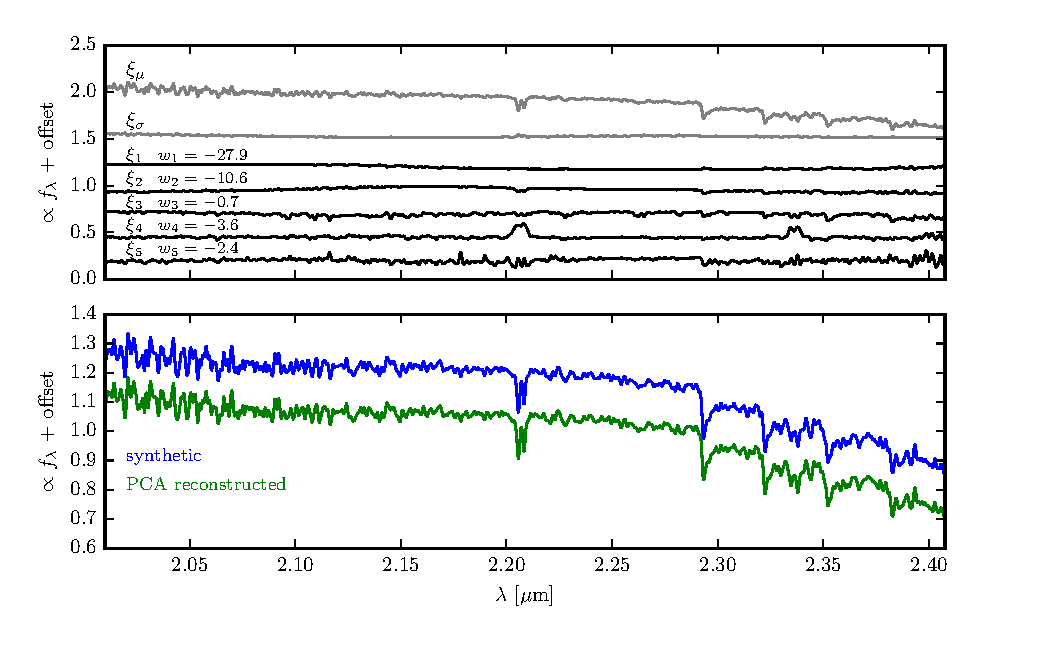
\includegraphics{figs/pca_reconstruct.pdf}
  \vspace{-0.6cm}
  \figcaption{ (\emph{top}) The mean spectrum, standard deviation spectrum, and five eigenspectra 
that form the basis of the \textsc{Phoenix} synthetic library used to model Gl~51, generated using 
a subset of the parameter-space most relevant for M dwarfs.  (\emph{bottom}) The original synthetic 
spectrum from the \textsc{Phoenix} library compared with a spectrum reconstructed from a linear 
combination of the derived eigenspectra using Eqn~\ref{eqn:reconstruct} (with the weights $w_k$ 
listed in the top panel figure).  \label{fig:pca_reconstruct}}
  \end{center}
\end{figure*}

The first step in designing a spectral emulator is to break down the library into an appropriate 
basis \citep{habib07, heitmann09}.  We chose the principal component basis to decompose the library 
into a set of ``eigenspectra", following the techniques of \citet{ivezic13}.  Prior to this 
decomposition, we isolate a subset of the library (containing $M$ spectra) with parameter values 
that will be most relevant to the target being considered (e.g., for Gl~51, this means considering 
only effective temperatures below $\sim$3800\,K).  We then standardize these spectra by subtracting 
off their mean spectrum and then ``whitening" them by dividing off the standard deviation spectrum 
measured in each pixel across the grid.  The mean spectrum is 
\begin{equation}
  \xi_\mu = \frac{1}{M} \sum_{i = 1}^M f_\lambda(\{\vt_\ast \}^\textrm{grid}_i)
\end{equation}
and the standard deviation spectrum is
\begin{equation}
  \xi_\sigma = \sqrt{\frac{1}{M} \sum_{i=1}^M \bigl [ f_\lambda(\{\vt_\ast \}^\textrm{grid}_i) - \xi_\mu \bigr]^2 }, 
\end{equation}
where $\{\vt_\ast \}^\textrm{grid}$ denotes the full collection of the $M$ sets of stellar 
parameters under consideration in the library and $\{\vt_\ast \}^\textrm{grid}_i$ denotes a single 
set of those parameters drawn from this collection.  In effect, all library spectra are 
standardized by subtracting the mean spectrum and dividing by the standard deviation spectrum
\begin{equation}
  \hat{f}_\lambda(\{\vt_\ast \}^\textrm{grid}) = \frac{f_\lambda(\{\vt_\ast \}^\textrm{grid}) - \xi_\mu}{\xi_\sigma}.
\end{equation}

The eigenspectra are computed from this standardized grid using principal component analysis 
\citep[PCA;][]{ivezic13}.  We decided to truncate our basis to the first $m$ eigenspectra, where 
$m$ is decided by the minimum number of eigenspectra required to reproduce any spectrum in the grid 
to better than 2\% accuracy for all pixels (the mean pixel error is generally much smaller than 
this, $\lesssim 0.5\%$).  We denote a single $N_{\rm pix}$-dimensional eigenspectrum as $\xi_k$, 
with principal component index $k = \{1, 2, \ldots, m\}$.  As an example, the eigenspectra basis 
computed for Gl~51 using the \textsc{Phoenix} library is shown in the top panel of 
Figure~\ref{fig:pca_reconstruct}.

\begin{figure*}[!t]
\begin{center}
  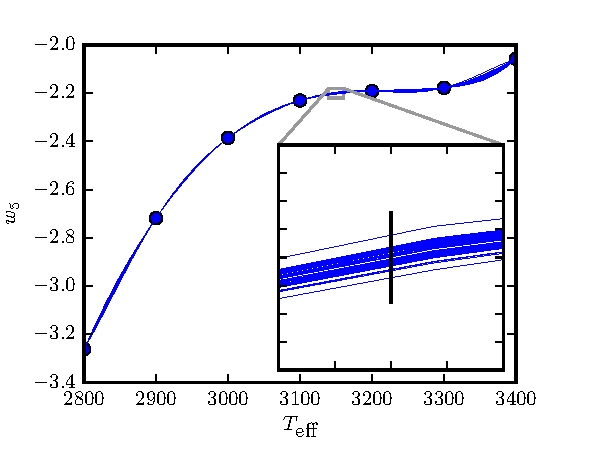
\includegraphics{figs/GP_left.pdf}
  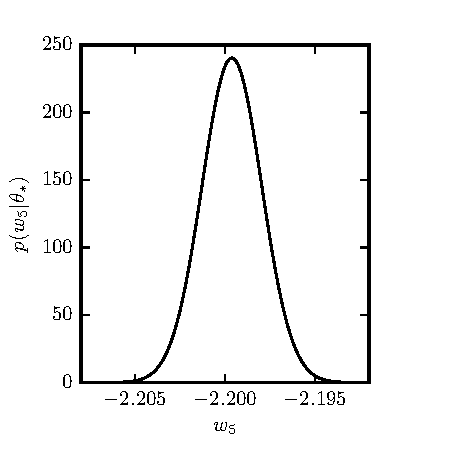
\includegraphics{figs/GP_right.pdf}
  \figcaption{The Gaussian process modelling of the principal component weights for the Gl51 \textsc{Phoenix} spectral library. (\emph{left}) the blue dots mark the weights $\mathbf{w}_5^\textrm{grid}$ of the 5th eigenspectrum $\xi_5$ computed at a one-dimensional slice of the spectral library for grid points with $\log g = 5.0$, $\Z = 0.0$ and various values of $T_\textrm{eff}$. In reality, the weights are a three-dimensional function of $\vt_\ast$. The thin blue lines show 50 random draws of possible functional forms described by the Gaussian process, constrained to pass through the grid weights. (\emph{inset}) a zoomed portion showing the scatter in the possible functional forms. The black vertical line represents a slice through the scatter of the predicted weight value at $\vt_\ast = [T_\textrm{eff} = 3150\,\textrm{K}, \log g = 5.0\,\textrm{dex}, \Z = 0.0\, \textrm{dex}]$. (\emph{right}) The posterior probability of $w_k$ at this value of $\vt_\ast$ is completely described by Eqn~\ref{eqn:conditional_gp}, allowing us to analytically marginalize over all probable values of the weights, and thus marginalize over all probable spectral interpolations.
\label{fig:GP_interp}}
\end{center}
\end{figure*}

Using the principal component basis, we can lossily reconstruct any spectrum from the library with 
a linear combination of the eigenspectra
% Is "lossily" really a word?  If so, wtf does it mean?
\begin{equation}
  f_\lambda(\{\vt_\ast \}^\textrm{grid}_i) \approx \xi_\mu + \xi_\sigma \sum_{k=1}^m w_k(\{\vt_\ast \}^\textrm{grid}_i) \, \xi_k
  \label{eqn:reconstruct}
\end{equation}
where $w_k$ is the weight of the $k^{\rm th}$ eigenspectrum.  These weights are 3-dimensional 
scalar functions that depend on the stellar parameters $\vt_\ast$.  These weights, which are 
generally smooth functions of the stellar parameters (see the left panel of 
Figure~\ref{fig:GP_interp}), can be determined at any grid point in the library by taking the dot 
product of the standardized synthetic spectrum with the eigenspectrum  
\begin{equation}
  w_k(\{\vt_\ast \}^\textrm{grid}_i) = \sum_\lambda \hat{f}_\lambda(\{\vt_\ast \}^\textrm{grid}_i) \, \xi_k.
\end{equation}
To simplify notation, we can write the collection of eigenspectra weights in a length-$m$ column 
vector
\begin{equation}
  \mathbf{w}(\vt_\ast) = 
  \begin{bmatrix}
    w_1(\vt_\ast )\\
    w_2(\vt_\ast )\\
    \vdots\\
    w_m(\vt_\ast )
  \end{bmatrix}
\end{equation}
and horizontally concatenate the eigenspectra into a matrix with $N_{\rm pix}$ rows and $m$ columns
% Christ, you know your paper's a mess when you start throwing around capital xi's.
\begin{equation}
  \mathbf{\Xi} = 
  \begin{bmatrix}
    \xi_1 & \xi_2 & \cdots & \xi_m \\
  \end{bmatrix} .
\end{equation}
Then, we can rewrite Eq.~(\ref{eqn:reconstruct}) as
\begin{equation}
  f_\lambda(\{\vt_\ast \}^\textrm{grid}_i) \approx \xi_\mu + \xi_\sigma \, \mathsf{I}_{N_{\rm pix}} \, \mathbf{\Xi} \, \mathbf{w}(\{\vt_\ast \}^\textrm{grid}_i)
  \label{eqn:reconstruct2}
\end{equation}
where $\mathsf{I}_{N_{\rm pix}}$ is an $N_{\rm pix} \times N_{\rm pix}$ identity matrix. 

To recapitulate, the framework described above can be used to decompose the synthetic spectra in a 
model library into a principal component basis, allowing us to lossily reconstruct any spectrum in 
the library as a (weighted) linear combination of $m$ eigenspectra.  The weights corresponding to 
each eigenspectrum are moderately-smooth scalar functions of the three stellar parameters, 
$\vt_{\ast}$.  Therefore, to create a spectrum corresponding to an arbitrary set of these 
parameters that is not in the spectral library, we must interpolate the weights to this new set.  
In practice, it may be possible to use a traditional scheme like spline interpolation to do this 
directly.  However, we found that with sensitive spectra (e.g., for Gl~51 the S/N is $>$400), the 
uncertainty in the interpolated representation of the spectrum can constitute a significant portion 
of the total uncertainty budget.  This, combined with the under-sampling of the synthetic grid can 
cause artificial ``peaking" of the posterior near grid points in the synthetic library, because the 
interpolated spectrum is not as good as the raw spectrum at the grid point.  Even explicitly 
accounting for interpolation error by doing ``drop-out" interpolation tests and empricially 
propagating it forward does not relieve this ``peaking" issue.  So instead, we address this problem 
by employing a Gaussian process to model the interpolation of the eigenspectra weights over 
$\vt_{\ast}$, thereby encapsulating the range of possible interpolated spectra. 

Each weight is modeled independently, so there is a new Gaussian process for each eigenspectrum.  
For a single eigenspectrum with index $k$, we denote the collection of 
$w_k(\{\vt_\ast \}^\textrm{grid}_i)$ evaluated for all the spectra in the library as 
$\mathbf{w}_k^\textrm{grid}$.  The Gaussian process treats $\mathbf{w}_k$ as a collection of random 
variables drawn from a joint multi-variate Gaussian distribution 
\citep{rasmussen05},
\begin{equation}
  \mathbf{w}_k^\textrm{grid} \sim \mathcal{N} \left ( \mathbf{0}, \mathbf{\Sigma}_k^\textrm{grid} \right ),
\end{equation}
with $\mathbf{\Sigma}_k^{\rm grid}$ denoting the covariances.  The kernel that describes the 
covariance matrix for this distribution is assumed to be a 3-dimensional squared exponential,
\begin{eqnarray}
  \mathcal{K}(\vt_i, \vt_j | \phi_{\rm int} ) &=& a_{\rm int}^2 \exp \left [ - \frac{(T_{\textrm{eff}_i} - T_{\textrm{eff}_j})^2}{2 \, \ell_{T_\textrm{eff}}^2 } \right] \nonumber \\
  & & \times \exp \left [-\frac{(\log g_i - \log g_j)^2}{2 \, \ell_{\log g}^2} \right ] \\
  & & \times \exp \left [ -\frac{ (\Z_i - \Z_j)^2}{2 \, \ell_{\Z}^2} \right ] \nonumber,
\end{eqnarray}
with hyper-parameters $\phi_{\rm int} = \{a_{\rm int}$, $\ell_{T_{\rm eff}}$, $\ell_{\log g}$, 
$\ell_{\Z}$\} representing an amplitude and length scale for each dimension of $\vt_{\ast}$.  
Unlike the \matern\ kernel used in Section~\ref{sec:method} (which produces a more structured 
behavior reminiscent of the spectral residuals), this squared exponential kernel has a smooth 
functional form that better represents the behavior of the eigenspectra weights across the library 
grid, as demonstrated in Figure~\ref{fig:GP_interp}.  The $M\times M$-dimensional covariance matrix 
is 
\begin{equation}
\mathbf{\Sigma}_k^\textrm{grid} = \mathcal{K}( \{\vt_\ast \}^\textrm{grid}, \{\vt_\ast \}^\textrm{grid} | \, \phi_{\rm int}),
\end{equation}
the evaluation of the covariance kernel for all pairings of stellar parameters at library 
gridpoints.

The optimal values for the hyperparameters $\phi_{\rm int}$ are given by the multi-variate Gaussian 
probability distribution, called the marginal likelihood function or ``evidence" for the weights 
\citep{rasmussen05},
\begin{equation}
  p(\mathbf{w}_k^\textrm{grid} | \mathbf{\Sigma}_k^\textrm{grid} ) = \mathcal{N}\left (\mathbf{w}_k^\textrm{grid} \left | \; \mathbf{0}, \mathbf{\Sigma}_k^\textrm{grid} \right . \right ).
\end{equation}
Because $\mathbf{\Sigma}_k^\textrm{grid}$ is defined by the kernel $\mathcal{K}$ and its associated 
hyperparameters, this likelihood function is equivalent to $p(\mathbf{w}_k^\textrm{grid} |\; 
a_\textrm{int}, \ell_{T_\textrm{eff}},  \ell_{\log g}, \ell_{\Z})$.  By multiplying this with a 
suitable prior over $a_\textrm{int}$ and $\ell$, we can construct a posterior distribution for 
$\phi_{\rm int}$.  For computational efficiency, we optimize the hyperparameters by finding the 
peak of the posterior distribution with a downhill gradient algorithm and then consider 
$\phi_{\rm int}$ fixed.

Now the Gaussian process is fully specified and can be used to predict the values of the weights at 
any arbitrary set of stellar parameters $\vt_\ast$ by considering them drawn from the joint 
distribution 
\begin{equation}
  \begin{bmatrix}
    \mathbf{w}_k^\textrm{grid}\\
    w_k
  \end{bmatrix} \sim
  \mathcal{N} \left (
  \mathbf{0},
  \begin{bmatrix}
  \mathbf{\Sigma}_k^\textrm{grid} & \mathcal{K}( \{\vt_\ast \}^\textrm{grid}, \vt_\ast) \\
  \mathcal{K}(\vt_\ast, \{\vt_\ast \}^\textrm{grid}) & \mathcal{K}(\vt_\ast,\vt_\ast)
  \end{bmatrix}
  \right )
\end{equation}
where $\mathcal{K}( \{\vt_\ast \}^\textrm{grid}, \vt_\ast)$ represents a length-$M$ column vector 
evaluated pairwise with all values in $\{\vt_\ast \}^\textrm{grid}$ and the proposed value of 
$\vt_\ast$.  This vector is stacked horizontally next to $\mathbf{\Sigma}^\textrm{grid}$, and its 
transpose is stacked vertically underneath $\mathbf{\Sigma}^\textrm{grid}$.  The combination of all 
these products results in an augmented covariance matrix of size ($M + 1, M + 1$).  The probability 
distribution of $w_k(\vt_\ast)$ is given by the conditional Gaussian distribution 
\citep{rasmussen05}
\begin{equation}
  p(w_k |\; \{\vt_\ast \}^\textrm{grid}, \mathbf{w}_k^\textrm{grid}, \vt_\ast) =  \mathcal{N} \left ( w_k \Bigl | \Bigr . \,  \mu_k , \sigma_k \right ),
 \label{eqn:conditional_gp}
\end{equation}
where
\begin{equation}
 \mu_k =   \mathcal{K}(\vt_\ast, \{\vt_\ast \}^\textrm{grid}) (\mathbf{\Sigma}^{\textrm{grid}})^{-1} \mathbf{w}_k^\textrm{grid}
\end{equation}
and 
\begin{eqnarray}
  \sigma_k &=& \mathcal{K}(\vt_\ast,\vt_\ast) - \\
  & & \mathcal{K}(\vt_\ast, \{\vt_\ast \}^\textrm{grid}) (\mathbf{\Sigma}^{\textrm{grid}})^{-1} \mathcal{K}( \{\vt_\ast \}^\textrm{grid}, \vt_\ast) \nonumber.
\end{eqnarray}
% Should one of these be transposed?  

Though the notation is complex, the interpretation is straightforward: the probability distribution 
of $w_k$ is a univariate Gaussian distribution whose mean and variance are a function of 
$\vt_\ast$, conditional upon the (fixed) values of $\mathbf{w}_k^\textrm{grid}$ and the squared 
exponential hyperparameters (an example is shown in Figure~\ref{fig:GP_interp}, right panel).

If we desired an actual value of the interpolated weight, for example to reconstruct a model spectrum, we could simply draw a Gaussian random variable from the probability distribution in 
Eq.~(\ref{eqn:conditional_gp}).  However, because we now know the probability distribution of the 
weight as a function of $\vt_\ast$, we can rewrite our data likelihood function 
(Eq.~\ref{eqn:lnlikelihood}) in such a way that it is possible to analytically marginalize over all 
possible values of $w_k$, and thus all probable spectral interpolations. 

Next, we consider the combined $m$ Gaussian processes that describe the weights for each 
eigenspectrum collectively.  For a given $\vt_\ast$, these Gaussian processes deliver a collection 
of $m$ one-dimensional Gaussian probability distributions.  Because we have modeled each $w_k$ 
independently, the joint probability of the vector of weights $\mathbf{w}$ is simply a 
multidimensional Gaussian matrix with only the diagonal elements populated,
\begin{eqnarray} \label{eqn:weight_conditional}
  p(\mathbf{w} |\, \vt_\ast) &=& \mathcal{N} \left ( \mathbf{w} \left | \right . \mathbf{\mu}_\mathbf{w}, \mathbf{\Sigma}_\mathbf{w} \right ) \\ \nonumber
  & = & \mathcal{N} \left ( \mathbf{w} \left | 
  \begin{bmatrix}
    \mu_1 \\
    \vdots \\
    \mu_m \\
  \end{bmatrix},
  \begin{bmatrix}
    \sigma_1^2 & \ldots & 0 \\
    \vdots & \ddots & \vdots \\
    0 & \ldots & \sigma_m^2 \\
  \end{bmatrix}
  \right .
  \right).
\end{eqnarray}

Up until this point, we have described the reconstruction of a spectrum as a linear combination of 
the eigenspectra that characterize the synthetic library (Figure~\ref{fig:pca_reconstruct}).  But 
in practice, that reconstructed spectrum must be further post-processed as detailed in 
Section~\ref{subsec:postprocess}.  Fortunately, because convolution is a linear operation, we can 
first post-process the raw eigenspectra according to $\vt_{\rm obs}$, and then represent the 
reconstructed spectrum as a linear combination of these modified eigenspectra without loss of 
information.  Unfortunately, the Doppler shift and resampling operations are not linear operations, 
and there will be some loss of information when trying to approximate them in this manner.  
However, we find that in practice when the synthetic spectra are oversampled relative to the 
instrument resolution by a reasonable factor, the flux error due to resampling is smaller than 
0.2\%\ across all pixels, and thus any effect of that information loss is negligible.  For 
notational compactness, we let $\widetilde{\xi}_\mu$, $\widetilde{\xi}_\sigma$, and 
$\widetilde{\mathbf{\Xi}}$ represent the post-processed eigenspectra, with an implied dependence on 
the current values of the observational parameters ($\vt_\textrm{obs}$) and the polynomial nuisance 
parameters $(\phi_\mathsf{P})$.  Now, the model spectrum is specified conditional on the vector of 
eigenspectra weights as 
\begin{equation}
  \mathsf{M} \bigl | \bigr . \,\mathbf{w} = \widetilde{\xi}_\mu + \mathbf{X} \mathbf{w}
\end{equation}
where 
\begin{equation}
  \mathbf{X} = \widetilde{\xi}_\sigma I_{N_{\rm pix}} \widetilde{\mathbf{\Xi}}.
\end{equation}
Because the Gaussian process describes a probability distribution of the weights, we now have a probability distribution of possible (interpolated) models
\begin{equation}
  p(\mathsf{M} |\, \mathbf{w}) = p( \mathbf{w} |\, \vt_\ast)
\end{equation}
and the likelihood function (Eq.~\ref{eqn:likelihood}) is specified conditional on the weights,
\begin{equation}
  p( \mathsf{D} |\, \mathsf{M}) = p( \mathsf{D} |\, \mathbf{w}) = 
  \mathcal{N} \left ( \mathsf{D} |\, \widetilde{\xi}_\mu + \mathbf{X} \mathbf{w} , \mathsf{C} \right ).
  \label{eqn:likelihood_conditional}
\end{equation}

The final task of designing the spectral emulator is to combine this data likelihood function with the posterior distribution of the eigenspectra weights (Eq.~\ref{eqn:weight_conditional}) and then marginalize over the weights
\begin{equation}
  p(\mathsf{D} | \vt_\ast) = \int p(\mathsf{D} | \mathbf{w}) p( \mathbf{w} | \vt_\ast) d \mathbf{w}
  \label{eqn:marginal}
\end{equation}
such that we are left with a modified posterior distribution of the data that incorporates the 
range of probable interpolation values for the model.  To perform this multidimensional integral, 
we use a convenient lemma found in \citet[their Appendix A]{gelman13}: if the probability 
distributions of $\mathbf{w}$ and $\mathsf{D} | \mathbf{w}$ are specified conditionally as in 
Eq.~\ref{eqn:weight_conditional} and \ref{eqn:likelihood_conditional}, respectively, then the 
marginal distribution (Eq.~\ref{eqn:marginal}) is
\begin{equation}
  p(\mathsf{D} | \vt_\ast, \vt_\textrm{obs}, \mathbf{\Phi}) = \mathcal{N} \left ( \mathsf{D} \bigl | \bigr .\, \widetilde{\xi}_\mu + \mathbf{X} \mathbf{\mu}_\mathbf{w}, \mathbf{X} \mathbf{\Sigma}_\mathbf{w} \mathbf{X}^T + \mathsf{C} \right),
\end{equation}
where the dependence on the model parameters is now made explicit.  We can couch this modified 
likelihood function in the form of Eqn~\ref{eqn:lnlikelihood} by rewriting
\begin{equation}
  \mathsf{M}^\prime = \widetilde{\xi}_\mu + \mathbf{X} \mathbf{\mu}_\mathbf{w}
\end{equation}
\begin{equation}
  \mathsf{R}^\prime = \mathsf{D} - \mathsf{M}^\prime 
\end{equation}
\begin{equation}
  \mathsf{C}^\prime = \mathbf{X} \mathbf{\Sigma}_\mathbf{w} \mathbf{X}^T + \mathsf{C}
\end{equation}
where $\mathsf{M}^\prime$ can be thought of as the ``mean model spectrum" given the model 
parameters, and the covariance matrix has been modified to account for the various probable 
manifestations of the model spectrum about that mean spectrum.

\bibliographystyle{yahapj}
\bibliography{stellarspectra}


\end{document}
